\begin{displayquote}
	
	\textsf{Facing the challenges of numerical linear algebra methods on a large-scale machine discussed in Section \ref{Krylov Subspace Methods}, the new programming model should be proposed with well-suited characteristics on modern architectures. These features include optimized communications, asynchronicity, diversity of natural parallelism and fault tolerance. In such numerical methods, the avoidance of operations involving synchronous communications is most important. Consequently, large scalar products and overall synchronization, and other operations involving communications between all cores have to be avoided. On the other hand, asynchronicity of communications has to be promoted. Indeed, this kind of communications could allow overlapping the computation operations inside a task and the tasks constituting theses methods. The diversity of natural parallelism existing in such methods can be exploited to take advantage of heterogeneity of targeted architectures. Fault tolerance and reusability should be also important integral parts of these methods. These characteristics allow the improvement of the performance of applications built on the basis of existing methods. In this chapter, we present an asynchronous distributed and parallel Unite and Conquer GMRES/LS-ERAM (UCGLE) method to solve sparse non-Hermitian systems on large platforms. The key feature of UCGLE comparing with the classical hybrid methods using LS polynomial preconditioner \cite{essai1999heterogeneous,he2006hybrid} that we presented in Section \ref{Preconditioning by Polynomials - Introduction in detail on Least Squares Polynomial method} is its distributed and parallel asynchronous communication and the manager engine implementation among three components, which are specified for the extreme-scale supercomputing platforms. We summarize the UC approach in Section \ref{Unite and Conquer approach}. In Section \ref{Iterative Methods based on UC Approach}, we analyze the possibility to construct different iterative methods based on UC approach. The theoretical parts of UCGLE are given in Section \ref{Asynchronous Unite and Conquer GMRES/LS-ERAM Method}. In Section \ref{Distributed and Parallel Implementation}, we present its distributed and parallel implementation, including the computing components, the manager engine, and the asynchronous communications. The experimental results on different supercomputers which evaluate the convergence, the parameters, the impact of spectral distribution, the scalability, and the fault tolerance are shown in Section \ref{Experiment and Evaluation}.}
\end{displayquote}

\vspace{0.6in}

\section{Unite and Conquer approach}\label{Unite and Conquer approach}

In general, UC approach is to make the collaboration of several iterative methods to accelerate the convergence of one of them. This approach is a model for the design of numerical methods by combining different computation components to work for the same objective, with asynchronous communication among them. \textit{Unite} implies the combination of different calculation components, and \textit{conquer} represents different components work together to solve one problem. Different independent components with asynchronous communications can be deployed on various platforms such as P2P, cloud and the supercomputer systems. 

The MERAM \cite{emad2005multiple} is an example of UC approach to solving eigenvalues based on an ERAM with multiple projections. This method projects an eigenproblem on a set of subspaces and thus creates a whole range of differently parameterized ERAM processes which cooperate to compute a solution of this problem efficiently. As shown in Fig. \ref{meram}, in MERAM, the restarting vector of each ERAM is updated by taking into account the interesting eigen-information obtained by the other ones. In details, the ERAM processes of a MERAM begin with several subspaces spanned by a set of initial vectors and a set of subspace sizes. If the convergence does not occur for any of them, then the new subspaces will be defined with initial vectors updated by taking into account the intermediary solutions computed by all the ERAM processes. In order to overcome the storage dependent shortcoming of ERAM, a constraint on the subspace size of each ERAM is imposed. As shown in Fig. \ref{meram-perf}, which is an experimental results extracted from \cite{emad2005multiple}, MERAM is able to accelerate the convergence of ERAM. The numerical experiments have demonstrated that this variant of MERAM is often much more efficient than ERAM. 

\begin{figure}[htbp]
	\centering
	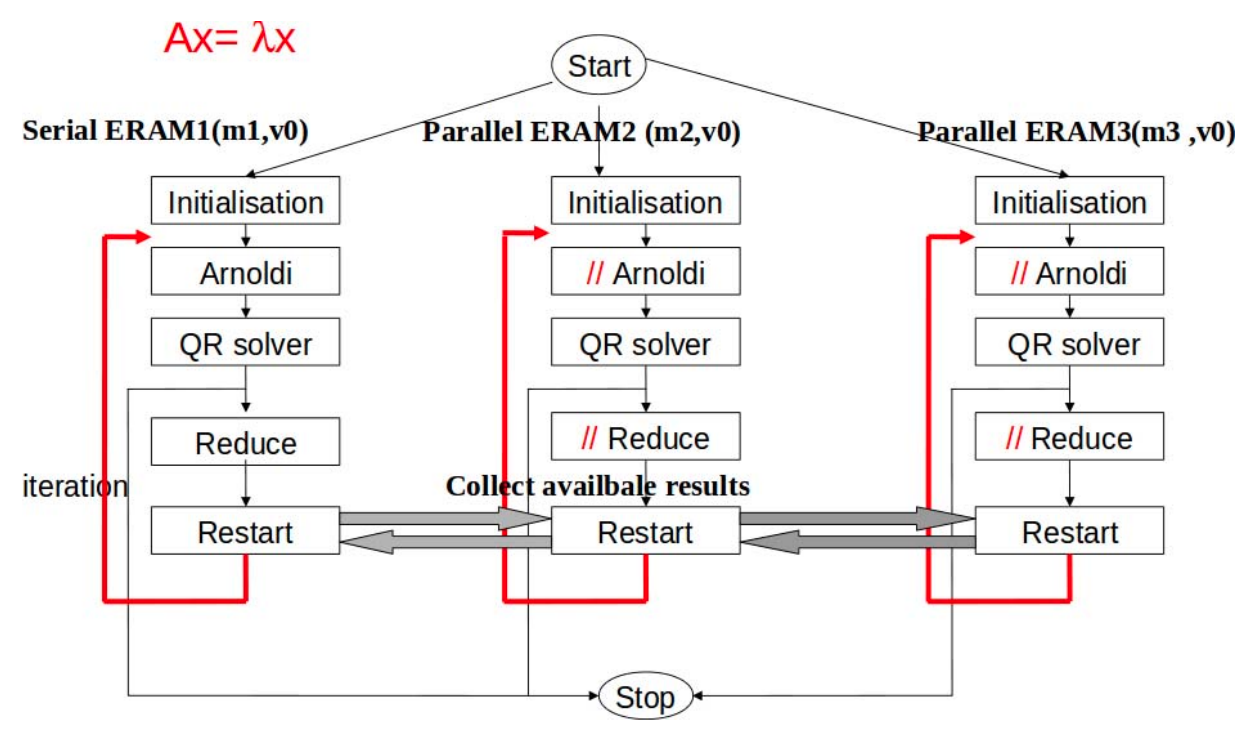
\includegraphics[width=6.3in]{fig/meram.png}
	\caption{An overview of MERAM \cite{emad2005multiple}.}
	\label{meram}
\end{figure}

\begin{figure}[t]
	\centering
	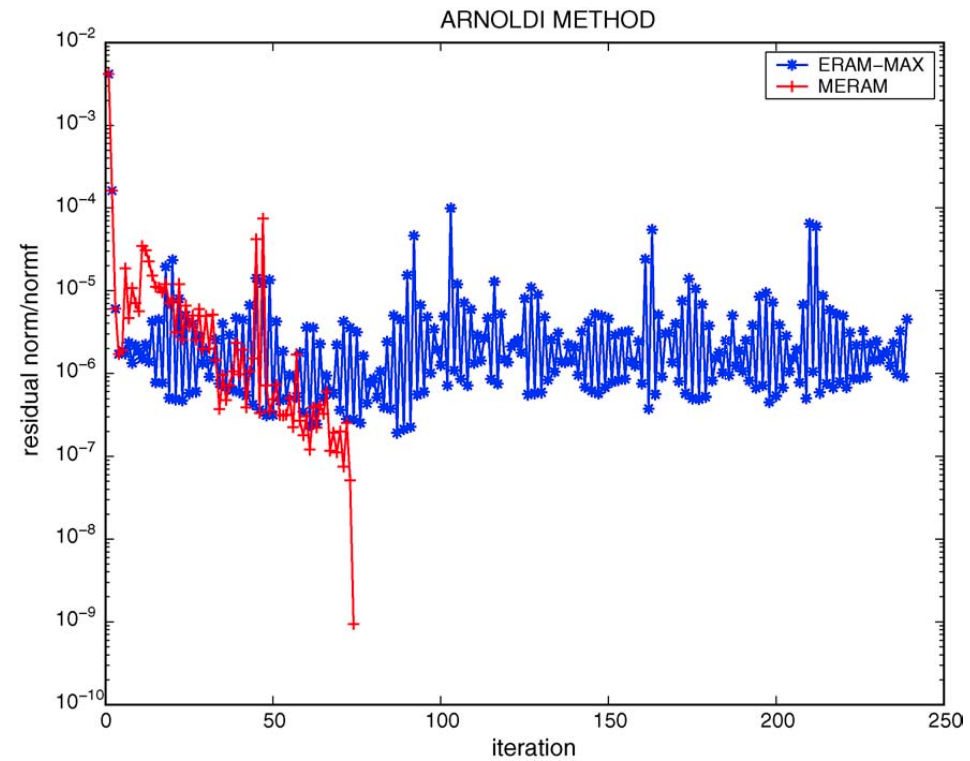
\includegraphics[width=6.2in]{fig/meram_perf.png}
	\caption{An example of MERAM: MERAM(5,7,10) vs. ERAM(10) with af 23560.mtx matrix. MERAM converges in 74 restarts, ERAM does not converge after 240 restarts \cite{emad2005multiple}.}
	\label{meram-perf}
\end{figure}

\section{Iterative Methods based on UC Approach}\label{Iterative Methods based on UC Approach}

 Based on the UC approach, most of the hybrid and deflated iterative methods are able to be transformed into distributed and parallel scheme by separating them into different computational components. In this section, we analyze the possibility to construct different iterative methods based on UC approach.

\subsection{Preconditioning Techniques}

As presented in Section \ref{Preconditioners for GMRES}, if Krylov subspace size $m$ is very large, iterative methods are often restarted after some iterations, to avoid enormous memory and computational requirements. One weakness of restarted methods is the lack of numerical robustness. They are likely to suffer from slow convergence for some problems. Different preconditioning techniques are applied to accelerate the convergence.

\subsubsection{Preconditioning by Matrix}

The first alternative is to use the preconditioning matrix $M$, and replace the original system by $Mx=b$, which is much easier to be solved. $M$ can be applied to the original systems either by the left, right or split preconditioning. Well-known preconditioners include SOR, Jacobi, AMG, ILU, etc.

\subsubsection{Preconditioning by Deflation}

It is not always true, but the convergence of Krylov subspace methods for solving linear systems depends on the distribution of eigenvalues. The removing or deflation of small eigenvalues might greatly improve the convergence performance. Hence deflated preconditioners should be constructed for each cycle of the restart. The small eigenvalues can be explicitly or implicitly deflated, e.g., the former uses the approximated Ritz pairs from $H_m$ to construct new restart residual vectors for linear solvers; the latter implicitly deflates these eigenvalues by special operations on $H_m$ and $V_m$ \cite{erhel1996restarted,burrage1998deflation,morgan2002gmres}. For example, a deflated GMRES introduced in \cite{morgan2002gmres}, firstly it approximates $k$ smallest eigenpairs of $H_m+\beta H_m^{-T}e_me_m^T$, secondly these eigenpairs are used to construct new $H_m$ and $V_m$ with the implicit deflation of these smallest eigenvalues.

The iterative methods for solving eigenvalue problems can be explicitly deflated by the Ritz values and vectors approximated through previous Arnoldi reduction procedures. ERAM uses the Ritz pairs to construct a new restart vector, which can deflate the gotten eigenvalues and accelerate the convergence. Two well-known implicitly deflated Krylov subspace methods for eigenvalue problems are IRAM and Krylov-Schur method \cite{stewart2002krylov}, which remove the unwanted eigenvalues implicitly by QR factorization and Krylov-Schur decomposition, respectively.

\subsubsection{Preconditioning by Polynomial}

In order to approximate a solution of linear system (\ref{ax=b1}), one approach is to get the inverse of $A$, denote it as $A^{-1}$, and then an approximate solution can be easily obtained as $\tilde{x}=A^{-1}b$. $\tilde{x}$ can be applied as a new residual vector for the subsequent restart, that is the polynomial preconditioning for linear solvers. In details, the cycle step of iterative methods is able to construct a Hessenberg matrix $H_m$ by the Arnoldi reduction. Then some dominant eigenvalues are approximated through the Ritz values of $H_m$. The preconditioning step is to get the best polynomial $p_k$ by these Ritz values, and $p_k$ is used to generate a new  $\tilde{x}$ for the next time restart of iterative methods.

The idea of polynomial preconditioning for the iterative solvers of eigenvalue problems is similar to the one for linear systems. In details, a selected polynomial $p_k$ can be constructed by the set of unwanted eigenvalues and new gotten Ritz values from previous Arnoldi reduction, and the operator $A$ can be replaced by $B_k=p_k(A)$. This polynomial is able to amplify the wanted eigenvalues of $A$ into the eigenvalues of $B_k$ with much larger norms comparing with other remaining eigenvalues, which will result in much faster convergence. The eigenvalues of $A$ can be obtained from the ones of $B_k$ by a Galerkin projection. The polynomial $p_k$ can be formulated either by the Chebyshev basic with the best ellipse constructed by the unwanted eigenvalues\cite{saad1987least}, or by a polygon refined with these unwanted eigenvalues \cite{manteuffel1977tchebychev}.

\subsubsection{Preconditioning by Shift-Invert}

Classic Krylov method is able to approximate the dominant eigenvalues. If the wanted values are not dominant, it is necessary to enlarge the Krylov subspace size, which requires larger memory and computational operations. One of the most effective techniques for solving such problems is to iterate with the shifted and inverted matrix $(A-\sigma I)^{-1}$. The eigenvalues approximated by this new operator are the ones around the given shift $\sigma$. Different fractions of eigenvalues can be efficiently calculated by changing $\sigma$.

\subsection{Analysis}

Table \ref{eigeninfor} summarizes the required information for the deflated, polynomial and Shift-Invert preconditioners of linear and eigensolvers. For the explicit deflation of iterative methods, the Ritz pair obtained from $H_m$ are used to perform the preconditioning. The explicitly deflated solvers use directly the Hessenberg matrix $H_m$ and the orthonormal basis of Krylov subspace $V_m$ to accelerate the convergence. The polynomial preconditioners for solving linear systems use the dominant eigenvalues approximated from $H_m$ to construct the best polynomial, and the unwanted Ritz values to formulate the preconditioning polynomial for solving eigenvalue problems. A special Shift-Invert preconditioner for eigenvalue problems is able to quickly approximate different parts of eigenvalues by selecting different shift value $\sigma$. The preconditioners implemented based on matrices is not listed in Table \ref{eigeninfor}.


\begin{table}[htbp]
	\renewcommand{\arraystretch}{1.4}
	\normalsize
	\caption{Information used by preconditioners to accelerate the convergence.}
	\centering
	\begin{tabular}{c|c|c}
		\toprule
		\cellcolor{gray!50}\diagbox{Precond}{Info}{Solver} & \cellcolor{gray!50}Linear Solver & \cellcolor{gray!50}Eigen Solver \\
		\midrule
		Explicit Deflation  &Ritz values and vectors& Ritz values and vectors \\
		\cellcolor{gray!20}Implicit Deflation  &\cellcolor{gray!20}	$H_m$ and $V_m$& \cellcolor{gray!20}$H_m$ and $V_m$ \\
		polynomial &Dominant Ritz values &unwanted Ritz values  \\
		\cellcolor{gray!20}Shift-Invert & \cellcolor{gray!20}\textcolor{red}{$\times$} &  \cellcolor{gray!20}shift value $\sigma$   \\
		\bottomrule
	\end{tabular}
	\label{eigeninfor}
\end{table}

\subsection{Separation of Components}

As presented in Section \ref{Toward Extreme Computing, Some Correlated Goals}, iterative methods for solving linear systems and eigenvalue problems on extreme-scale platforms should be modified and optimized by minimizing global communication, reducing synchronization points, and promoting asynchronicity. Recent studies have focused more on the optimization of different parts inside iterative methods, e.g., the communication avoiding techniques for linear algebra operations \cite{hoemmen2010communication, carson2015communication} and pipelined strategies for Krylov methods \cite{morgan2016stochastic, cools2017communication}. Since modern supercomputers can be seen as special Grid computers, it is necessary to divide the applications into different complex components according to their functionalities. They should be implemented with asynchronous communications and controlled by a manager engine. The first step is to identify different components of preconditioned iterative methods.

\subsubsection{Component Identification inside Iterative Methods}

Based on Table \ref{eigeninfor}, the mechanism to separate the numerical methods into different computation components is proposed. For the deflation and polynomial preconditioned iterative methods, the important information for the preconditioning is either $H_m$ and $V_m$ or the Ritz pairs obtained from $H_m$ and $V_m$.  Immediately, they can be divided into two parts: the solving and preconditioning parts. Moreover, a supplementary computational component should also be provided which is able to generate the information used by the preconditioners. Finally, these algorithms can be divided into three kinds of computation components:

\begin{itemize}
	\item \textit{Solver Component} for solving problems;
	\item \textit{Information Generator Component} to generate this information used by the preconditioners;
	\item \textit{Preconditioner Component} for the preconditioning pretreatment for the solvers.
\end{itemize}

Fig. \ref{fig:cyclic} gives a cyclic relation of the proposed three components for the deflation and the polynomial preconditioned methods, which communicate with each other by asynchronous communications. Various existing algorithms can be transformed into the three types of components, e.g., for the polynomial preconditioned solver for linear systems, three types of computation components are: 
\begin{enumerate}[label=(\arabic*)]
	\item an iterative method to solve the systems;
	\item an eigensolver to approximate the dominant eigenvalues;
	\item a preconditioning pretreatment component to generate the preconditioning parameters, either by the ellipse or the refinement of a polygon.
\end{enumerate}

and for the deflation preconditioned eigensolvers, three types of computation components are: 

\begin{enumerate}[label=(\arabic*)]
	\item an eigensolver to solve the problems; 
	\item another eigensolver with different settings (e.g., the Krylov subspace size, the shift value) to generate the information for preconditioning, such as $H_m$ and $V_m$ for the implicit deflation and Ritz pairs for the explicit deflation; 
	\item best preconditioning information can be selected by the \textit{Preconditioner Component} using the information of previous two components (e.g., for explicit deflation, the best information can be the combination of Ritz vectors from different components), and it can achieve the numerical performance better than conventional deflated iterative methods.
\end{enumerate}


\begin{figure}[htbp]
	\centering
	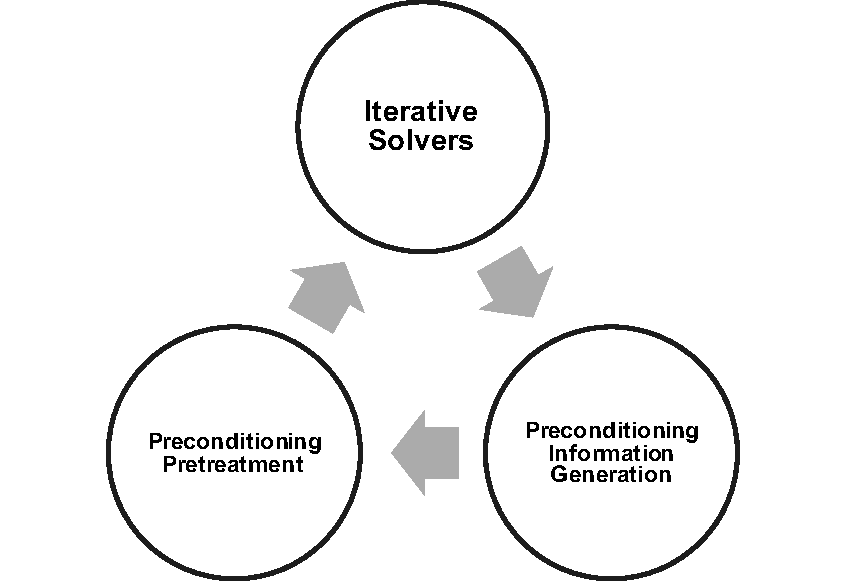
\includegraphics[width=0.8\linewidth]{fig/cyclic.pdf}
	\caption{Cyclic relation of three computational components.}
	\label{fig:cyclic}
\end{figure}

For the shift-invert preconditioned eigensolvers, they can be divided into several similar solvers with different shift value $\sigma$. These components can be tickly restarted with much smaller Krylov subspace size to approximate a small fraction of wanted eigenvalues. The total wanted ones can be a combination the subsets of different components. This is similar to the spectrum slicing strategies for restarted Lanczos methods introduced by Campos et al. \cite{campos2012strategies}.

For the matrix preconditioned methods, it is difficult to divide the solver and preconditioning matrix into two independent components with asynchronous communications, since the preconditioned matrix $M$ should be left or right multiplied with the operator $A$ for each time projection inside the Arnoldi reduction process, which cannot be explicitly separated. 

\subsubsection{Distributed and Parallel Implementation of Components}

By separating the preconditioned iterative methods into different components, they can be implemented in a distributed manner. These different components communicate with others by asynchronous communications. They can concentrate on their own tasks independently from other components unless the necessary data are asynchronously received from others. The synchronization points for the preconditioning can be covered, and the fault tolerance can be significantly improved. For each component, it can be replaced by the implementation with the linear algebra operations optimized by the recent research, which introduce a potential improvement for the parallel performance of each component. The separation of components makes it easier to take advantage of current research to optimize linear algebra operations within iterative methods, thereby improving the parallel performance of each computational component.

\subsubsection{Benefits of separating Components}

Dividing iterative methods into components with asynchronous communication introduces both numerical and parallel benefits for them.

\begin{itemize}
	\item \textit{Numerical benefits}: for conventional deflation and polynomial preconditioned methods, the information used is obtained from previous Arnoldi reduction, and it might be difficult to explore larger subspace. Therefore the convergence might be slowed down. For the methods implemented with the proposed paradigm, the solving and preconditioning parts are independent, thus for the \textit{Information Generator Components}, different Arnoldi reduction procedures can be implemented in the same time with much larger Krylov subspace or other parameters. This information applied to the deflation or polynomial preconditioned \textit{Solver Components} can be different from their own Arnoldi reduction, which improve the flexibility the algorithms, e.g., much more eigenvalues and larger searching space for the deflation. Hence the limitation of spectral information caused by restarting might be broken down, and faster convergence might be obtained. The numerical benefits for linear and eigensolver are already respectively discussed in \cite{Wu:2018:DPA:3149457.3154481} and \cite{emad2005multiple}.
	
	\item \textit{Parallel benefits}: parallel performance of iterative can be obtained by the promotion of asynchronization and reduction of synchronizations and global communications. Separating components improves also the fault tolerance and reusability of algorithms.
\end{itemize}

\section{Unite and Conquer GMRES/LS-ERAM Method}\label{Asynchronous Unite and Conquer GMRES/LS-ERAM Method}

In this section, we try to propose a new multi-level parallelism programming paradigm to solve linear systems based on the UC approach. We select the hybrid method preconditioned by the Least Squares polynomial to construct a distributed and parallel linear solver, that is the UCGLE method. Firstly, Section \ref{Divide of Linear Solvers into Components} present different computational components inside UCGLE. In Section \ref{UCGLE}, we give an implementation and workflow of UCGLE.

\subsection{Selection of Components} \label{Divide of Linear Solvers into Components}

In this section, we list the details for the three computational components in UCGLE as below,

\begin{enumerate}[label=(\arabic*)]
	\item \textit{Solver Component: }this component is implemented with restarted GMRES to solve non-Hermitian linear systems.
	\item  \textit{Information Generator Component: }the materials for Least Squares polynomial preconditioner are the dominant eigenvalues, thus this type of component is implemented with ERAM to approximate the eigenvalues. 
	\item \textit{Preconditioner Component: }this component is to generate the Least Squares polynomial preconditioning parameters using the approximated eigenvalues by the ERAM Component. In this paper, it is denoted as LSP component.
\end{enumerate}


\subsection{Workflow of UCGLE} \label{UCGLE}

In the conventional implementation of this hybrid method, the eigenvalues used to construct the least squares polynomials are computed by the Hessenberg matrix $H_m$ after each time Arnoldi reduction cycle of GMRES. In UCGLE, the linear solver, the approximation of eigenvalues and the construction of least squares polynomials are separated into three different parts. These three computing components work independently with each other, and they share the necessary information by the asynchronous communications.

UCGLE method composes mainly two parts: the first part uses the restarted GMRES method to solve the linear systems; in the second part, it computes a specific number of approximated eigenvalues, and then applies them to the Least Squares method and gets a new preconditioned residual, as a new initial vector for restarted GMRES. 

Figure \ref{fig:worflow} gives the workflow of UCGLE method with three computation components. ERAM Component and GMRES Component are implemented in parallel, and the communication among them is asynchronous. ERAM Component computes a desired number of eigenvalues, and then sends them to LSP Component; LSP Component uses these received eigenvalues to output a new residual vector, and sends it to GMRES Component; GMRES Component uses this residual as a new restarted initial vector for solving non-Hermitian linear systems.

\begin{figure}[t]
	\centering
	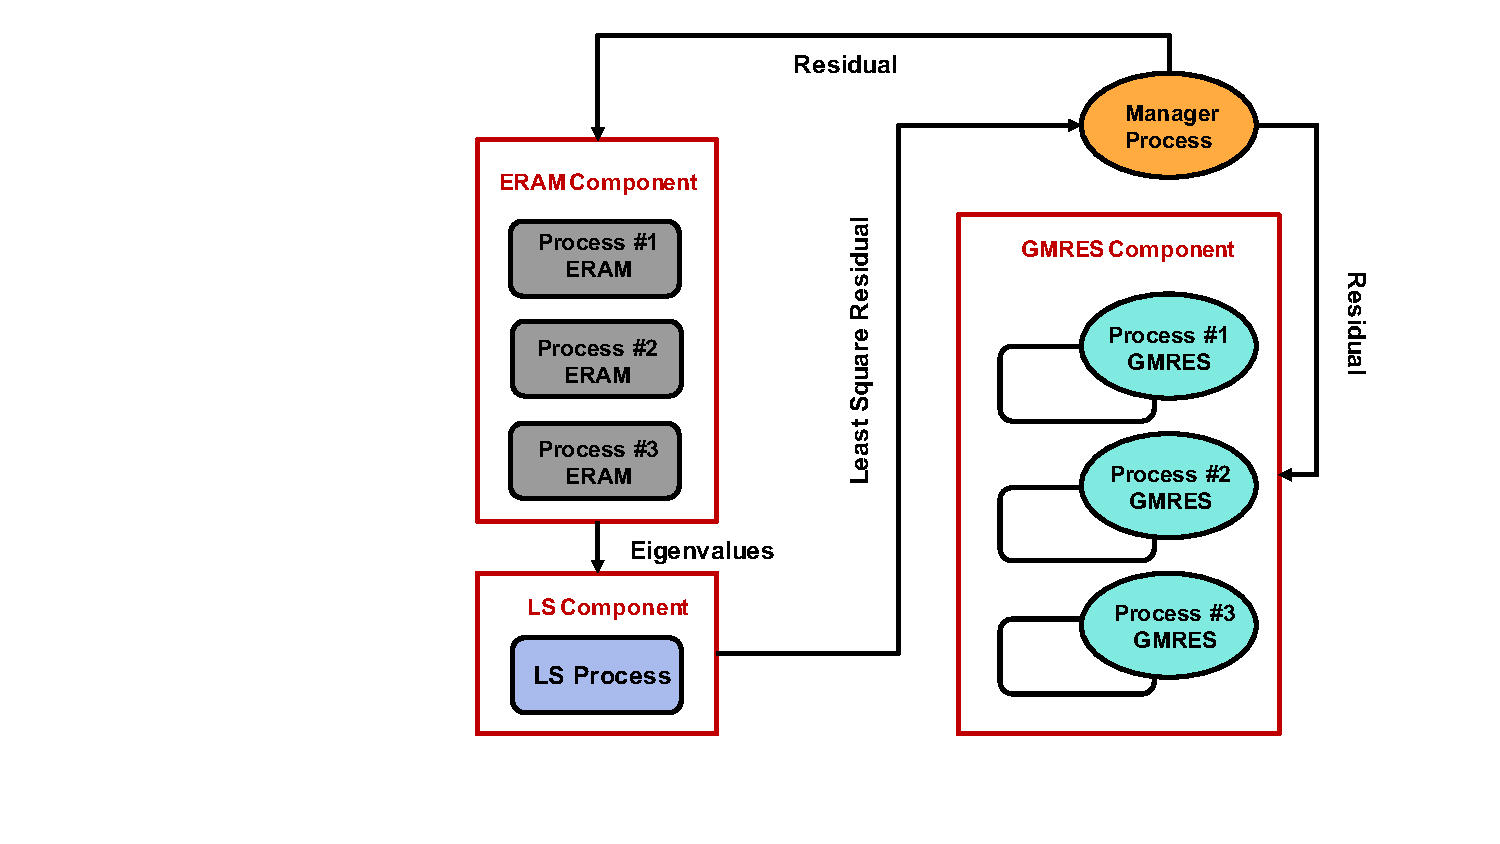
\includegraphics[width=0.99\linewidth]{fig/workflow.pdf}
	\caption{Workflow of UCGLE method.}
	\label{fig:worflow}
\end{figure}


\section{Distributed and Parallel Implementation}\label{Distributed and Parallel Implementation}

This section gives the distributed and parallel implementation, including the components, the multi-level parallelism, the manager engine, and the asynchronous communications.

\subsection{Component Implementation}

This section gives the basic implementation and workflow for each component in UCGLE, and Algorithm \ref{alg:gmres/ls-a} gives the implementation of UCGLE in details.

\subsubsection{GMRES Component}

GMRES Component aims to complete the solving a linear system $Ax=b$. It takes as input an operator matrix $A$ and two vectors, $x$ the initial guess vector and $b$ the related RHS. GMRES approximates the solution starting from this initial guess vector until the exact solution is found or if a stopping criterion is met, for example, that the residual norm is below a given threshold (e.g., $||r||_2 \leq 10e^{-8}$). In practice, GMRES are restarted after $m$ steps of iterations in order to reduce the memory requirement. Before each time of restart, GMRES Component check if it receives asynchronously the LSP parameters from LSP Component. If received, it will provide these parameters to generate a new residual vector and use it as the restart vector, if not, GMRES will be normally restarted. 

\begin{breakablealgorithm}
	\caption{Implementation of Components}   
	\label{alg:gmres/ls-a}   
	\begin{algorithmic}[1]
		\Function{LOADERAM}{$input$: $A, m_a, \nu, r, \epsilon_a$}
		\While{exit==False}
		\State ERAM($A, r, m_a, \nu,\epsilon_a$, $output$: $\Lambda_r$)
		\State Send ($\Lambda_r$) to LS
		\If{$saveflg==TRUE$} 
		\State write ($\Lambda_r$) to file $eigenvalues.bin$\EndIf
		\If{Recv ($X\_TMP$)} 
		\State update $X\_TMP$\EndIf
		\If{Recv ($exit==TRUE$)} 
		\State Send ($exit$) to LS Component  \State stop \EndIf
		\EndWhile
		\EndFunction
		\Function{LOADLS}{$input$: $A,b, d$}
		\If {Recv($\Lambda_r$)}
		\State LSP-Pretreatment{($input$: $A,b,d,\Lambda_r$, $output$: $A_d, B_d, \Delta_d, H_d$)}
		\State Send ($A_d, B_d, \Delta_d, H_d$) to GMRES Component
		\EndIf
		\If{Recv ($exit==TRUE$)} 
		\State stop \EndIf
		\EndFunction
		
		\Function {LOADGMRES}{$input$: $A, m_g, x_0, b, \epsilon_g, L, s_{use}$, $output$: $x_m$}
		\State $count=0$
		\State BASICGMRES{($input$: $A, m, x_0,b$, $output$: $x_m$)}
		\State $X\_TMP = x_m$
		\State Send ($X\_TMP$) to ERAM Component
		\If{$||b-Ax_m||<\epsilon_g$}
		\State \Return $x_m$
		\State Send ($exit==TRUE$) to ERAM Component
		\State Stop
		\Else \If{$count \mid L$}
		\If{recv ($A_d, B_d, \Delta_d, H_d$)}
		\State $r_0=f-Ax_0$, $\omega_1 = r_0$ and $x_0=0$
		\For {$k=1,2,\cdots, lsa$} \label{lsastart}
		\For {$i=1, 2, \cdots, d-1$}
		\State $\omega_{i+1}=\frac{1}{\beta_{i+1}}[A\omega_i-\alpha_i\omega_i-\delta_i\omega_{i-1}]$
		\State $x_{i+1}=x_i+\eta_{i+1}\omega_{i+1}$
		\EndFor
		\EndFor  \label{lsaend}
		\State set $x_0=x_d$, and GOTO 1
		\State $count++$
		\EndIf
		\Else
		\State set $x_0=x_m$, and GOTO 1
		\State $count++$
		\EndIf
		\EndIf
		\If{Recv ($exit==TRUE$)} 
		\State stop \EndIf
		\EndFunction
	\end{algorithmic}  
\end{breakablealgorithm}

Fig. \ref{gmres-component} gives the workflow of GMRES Component. GMRES Component loads the parameters $A, m_g, x_0, b, \epsilon_g, L, s_{use}$ to solve the linear systems. At the beginning of the execution, it behaves like the basic GMRES method. When it finishes the $m^{th}$ iteration, it will check if the condition $||b-Ax_m||<\epsilon_g$ is satisfied, if yes, $x_m$ is the solution of linear system $Ax=b$, or GMRES Component will be restarted using $x_m$ as a new initial vector. A parameter $count$ is used to count the times of restart. All these processes are similar to a Restarted GMRES. However, when $count$ is an integer multiple of $L$ (number of GMRES restarts between two times preconditioning of LS polynomial), it will check if it has received the parameters $A_d, B_d, \Delta_d, H_d$ from LS Component. If yes, these parameters will be used to construct a preconditioning polynomial $P_d$, which can be used to generate a preconditioned residual $x_d$, then set the initial vector $x_0$ as $x_d$, and restart the basic GMRES, until the exit condition is satisfied. The GMRES component has the role of solving the linear system.  We reused PETSc's GMRES implementation and modified it to include sending and receiving data and calculating the new residual. 

\begin{figure}[t]
	\centering
	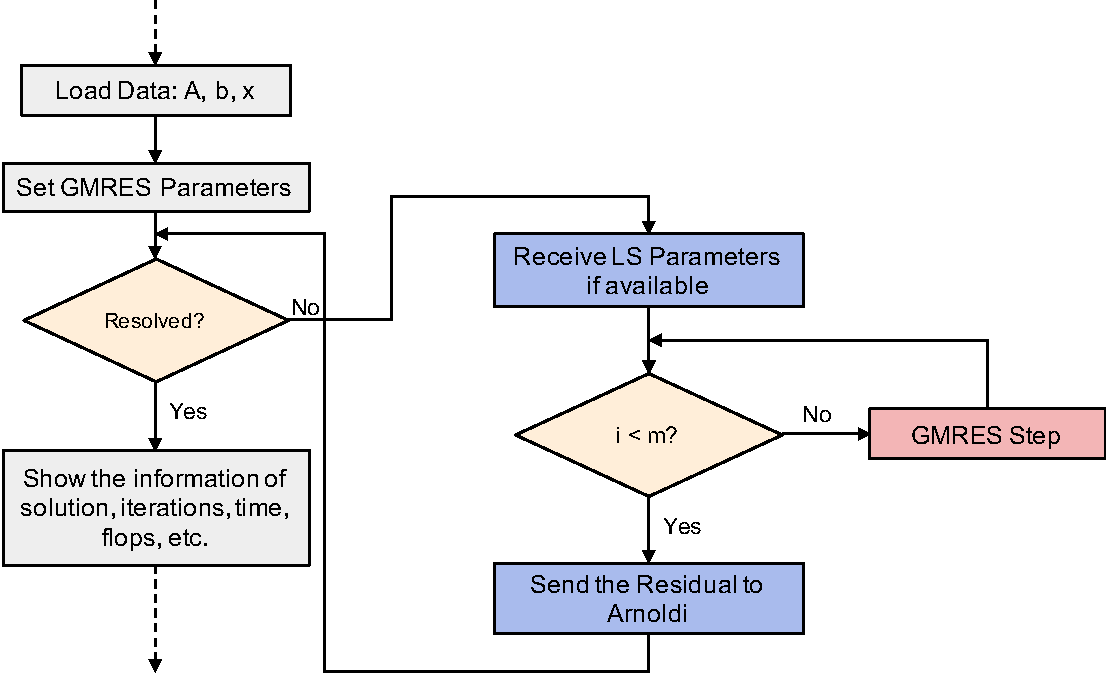
\includegraphics[width=0.99\linewidth]{fig/GMRES-component.pdf}
	\caption{GMRES Component.}
	\label{gmres-component}
\end{figure}

\subsubsection{ERAM Component}

\begin{figure}[t]
	\centering
	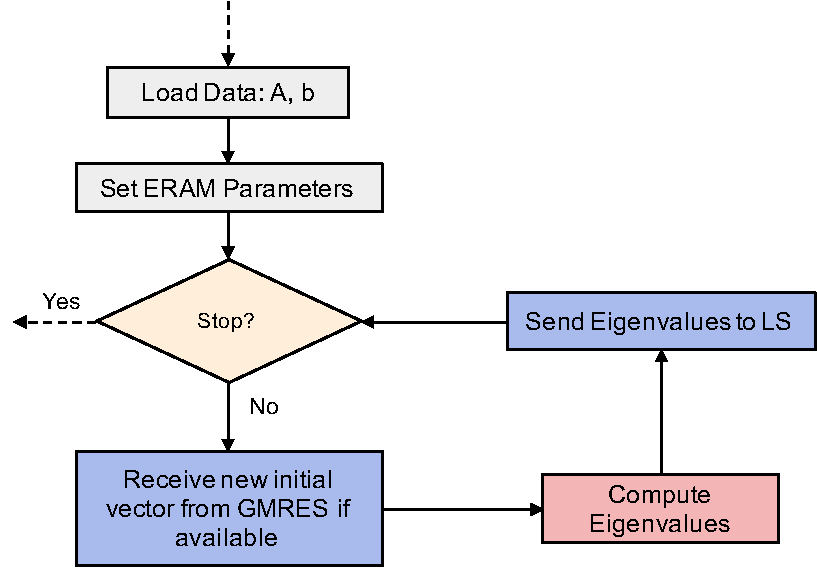
\includegraphics[width=0.8\linewidth]{fig/ERAM-component.pdf}
	\caption{ERAM Component.}
	\label{eram-component}
\end{figure}

Fig. \ref{eram-component} gives the workflow of ERAM Component. ERAM Component loads the parameters $m_a, v, r, \epsilon_a$ and the operator matrix $A$, then launches ERAM function. When it receives a new vector $X\_TMP$ from GMRES Component, this vector will be stored in ERAM Component. This vector is updated with the continuous receiving of a new one from GMRES Component. If the $r$ eigenvalues $\Lambda_r$ are approximated by ERAM Component, it will send them to LSP Component, at the same time, it is able to save the eigenvalues into the local file. We reused SLEPc's ERAM implementation by adding the sending and receiving functionalities.

\subsubsection{LSP Component}

Fig. \ref{ls-component} gives the workflow of ERAM Component. LSP Component won't start work until it receives the eigenvalues $\Lambda_r$ sent from ERAM Component. Then it will use them to compute the parameters $A_d, B_d, \Delta_d, H_d$, whose dimensions are related to LSP parameter $d$, the Least Squares polynomial degree, and send these parameters to GMRES Component. The Cholesky factorization inside LSP Component is implemented by the routine provided by LAPACK.

\begin{figure}[t]
	\centering
	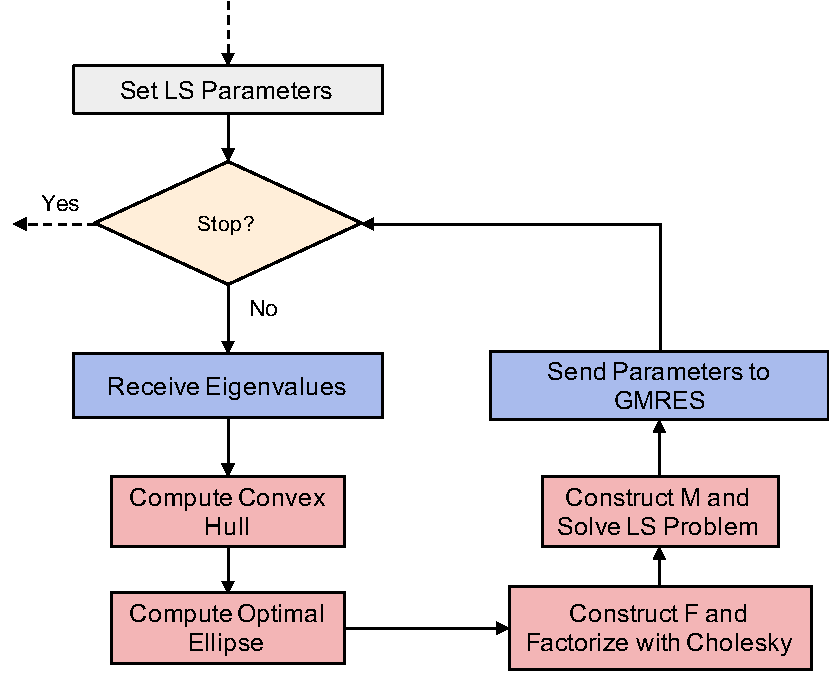
\includegraphics[width=0.8\linewidth]{fig/LS-component.pdf}
	\caption{LSP Component.}
	\label{ls-component}
\end{figure}

\subsection{Parameters Analysis} \label{parameter analysis}
\begin{figure}[h]
	\centering
	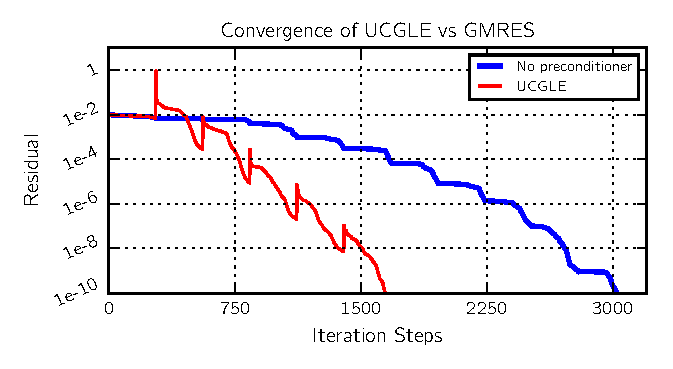
\includegraphics[width=6.2in]{fig/conv.eps}
	\caption{Convergence comparison of UCGLE method vs classic GMRES.}
	\label{fig:conv}
\end{figure}

UCGLE method is a combination of three different methods, there are a number of parameters, which have impacts on its convergence rate. We summarize these different related ones, and classify them according to their relations with different components.

\begin{enumerate}[]
	\item GMRES Component
	\begin{enumerate}[]
		\item $m_g$: GMRES Krylov Subspace size 
		\item $\epsilon_g$: absolute tolerance for  the GMRES convergence test
		\item $P_g$: GMRES core number
		\item $lsa$: number of times that polynomial applied on the residual before taking account into the new eigenvalues
		\item $L$: number of GMRES restarts between two times of LS preconditioning
	\end{enumerate}
	\item ERAM Component
	\begin{enumerate}[]
		\item $m_a$: ERAM Krylov subspace size
		\item $r$: number of eigenvalues required
		\item $\epsilon_a$: tolerance for the ERAM convergence test
		\item $P_a$: ERAM core number
	\end{enumerate}
	\item LSP Component
	\begin{enumerate}[]
		\item $d$: Least Squares polynomial degree
	\end{enumerate}
\end{enumerate}

\begin{figure}[t]
	\centering
	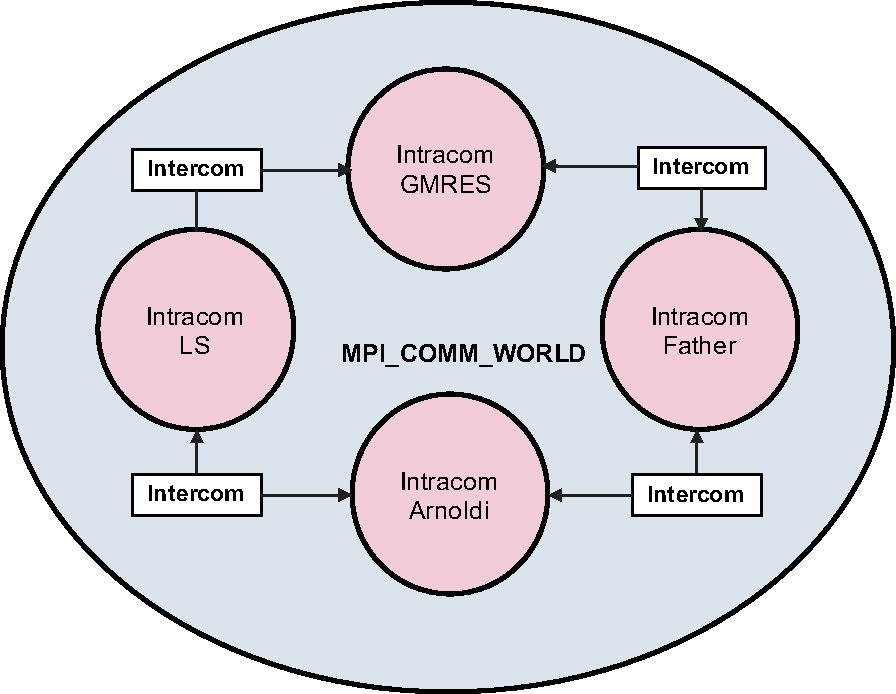
\includegraphics[width=0.72\linewidth]{fig/UCGLE_COMM_WORLD.pdf}
	\caption{Creation of Several Intra-Communicators in MPI.}
	\label{fig:ucgle_comm_world}
\end{figure}

Suppose that the computed convex hull by Least Squares contains eigenvalues $\lambda_1,\cdots, \lambda_m$, the residual given by Least Square polynomial of degree $d-1$ is

\[
r = \sum_{i=1}^{k}\rho_i R_d(\lambda_i)u_i + \sum_{i=m+1}^{n}\rho_i R_d(\lambda_i)u_i
\]

The first part of this residual is minimized by the Least Square polynomial method using the eigenvalues inside convex hull $H_k$, and the second part is large since the related eigenvectors associated with the eigenvalues outside $H_k$. With the number of approximated eigenvalues $d$ increasing, the first part will be much closer to zero and the second part keeps enormous. The next restart process of GMRES can be still accelerated since it restarts with the combination of eigenvectors. The more eigenvalues are known, the more significant acceleration will be. The convergence comparison of UCGLE and classic GMRES is given in Fig. \ref{fig:conv}. The large peaks appear in the UCGLE curve for each time restart. It means that the residual turns to be large, and then will drop down very quickly with the acceleration of LS polynomial method.

\subsection{Distributed and Parallel Manager Engine Implementation}\label{Distributed and Parallel Manager Engine Implementation}


The GMRES method has been implemented by PETSc, and the ERAM method is provided by SLEPc. Additional functions have been added to the GMRES and ERAM provided by PETSc and SLEPc in order to include the sending and receiving functions of different types of data. For the implementation of LSP Component, it computes the convex hull and the ellipse encircling the Ritz values of matrix $A$, which allows generating a novel Gram matrix $M$ of selected Chebyshev polynomial basis. This matrix should be factorized into $LL^T$ by the Cholesky algorithm. The Cholesky method is ensured by PETSc as a preconditioner but can be used as a factorization method. The implementation based on these libraries allows the recompilation of the UCGLE codes to adapt to both CPU and GPU architectures. The experimentation in this chapter does not consider the OpenMP thread level of parallelism since the implementation of PETSc and SLEPc is not thread-safe due to their complicated data structures. The data structures of PETSc and SLEPc makes it more difficult to partition the data among the threads to prevent conflict and to achieve good performance \cite{petsc-user-ref}.

\subsubsection{Implementation of the Inter-component Communication Network}

In order to establish different computational components with asynchronous communications, the first solution is to create several communicators inside of $MPI\_COMM\_WORLD$ and their inter-communication. The topology of communication among these groups is a circle shown in Figure \ref{fig:ucgle_comm_world}. The total number of computing units supplied by the user is thus divided into four groups according to the following distribution: $P_t$ is the total number of processes, then $P_t = P_g + P_a + P_l + P_m$, where $P_g$ is the number of processes assigned to GMRES Component, $P_a$ the number of processes to ERAM component, $P_l$ the number of processes allocated to LSP Component and $P_f$ the number of processes allocated to $Manager Process$ proxy. $P_g$ and $P_a$ are greater than or equal to $1$, $P_l$ and $P_m$ are both exactly equal to $1$. LSP Component is a serial component because the Least Squares polynomial method cannot be parallelized.

$P_t$ is thus divided into several MPI groups according to a color code. The minimum number of processes that our program requires is $4$. We utilize the mechanism of MPI standard to support the communication of our application fully. The communication layer that does not depend on the application, this allows the replacement and scalability of various components provided.

\subsubsection{Asynchronous Communication Mechanism}

\begin{figure}[t]
	\centering
	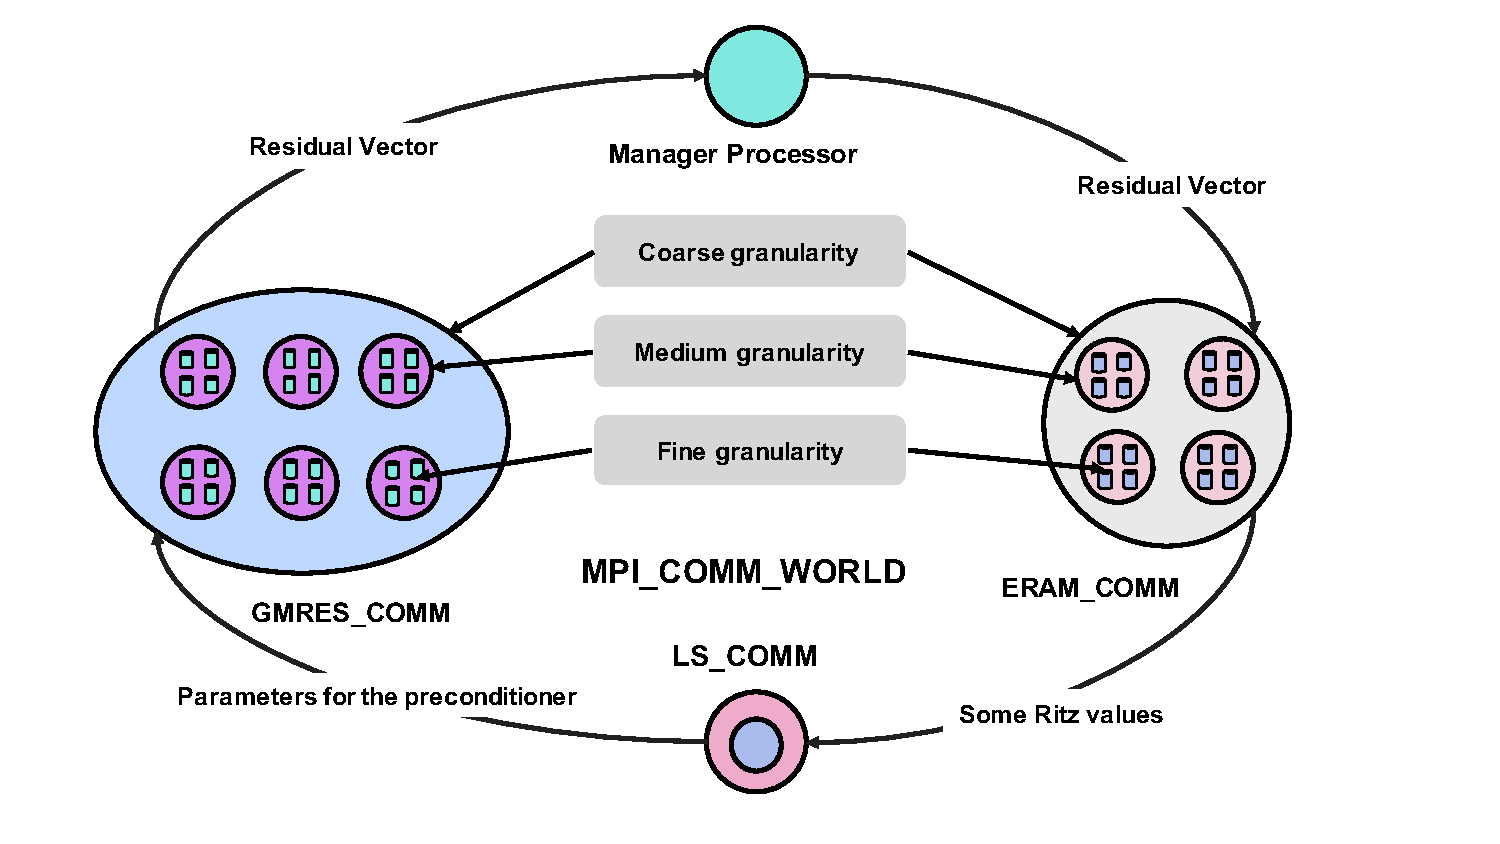
\includegraphics[width=0.9\linewidth]{fig/GLSA_MPI.pdf}
	\caption{Communication and different levels parallelism of UCGLE method}
	\label{fig:glsa_mpi}
\end{figure}

As shown in Figure \ref{fig:glsa_mpi}, UCGLE has three levels of parallelism which is suitable for the modern supercomputers. In fact, the main characteristic of UCGLE method is its asynchronous communication. But the synchronous communication takes place inside of GMRES and ERAM components. Distributed and parallel communication involves different types of exchange data, such as vectors, scalar arrays, and signals among different components. When the data are sent and received in a distributed way, it is essential to ensure the consistency of data. In our case, we choose to introduce an intermediate node as a proxy to carry out only several types of exchanges and thus facilitate the implementation of asynchronous communication. This proxy is called \textit{Manager Process} as in Figure \ref{fig:glsa_mpi}. One process can fulfill all the data exchanges.

\begin{figure}[htbp]
	\centering
	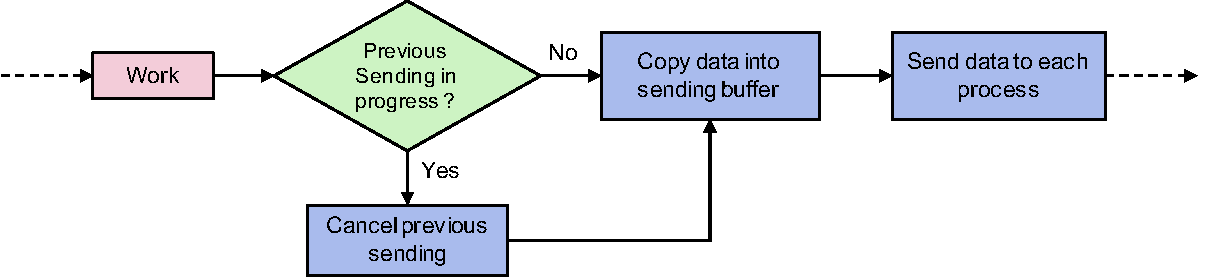
\includegraphics[width=6.2in]{fig/send.pdf}
	\caption{Data Sending Scheme from one group of process to the other.}
	\label{fig:send}
\end{figure}

\begin{figure}[t]
	\centering
	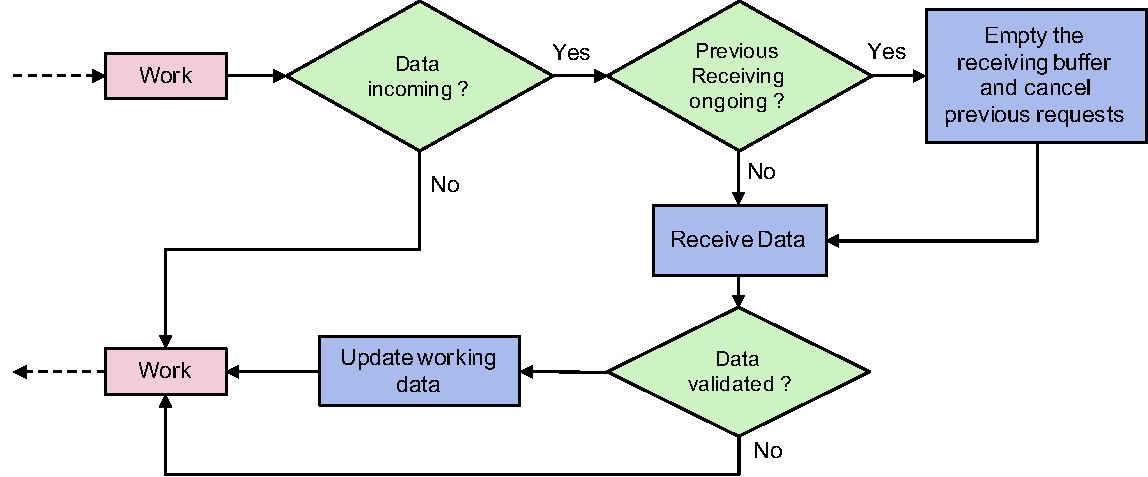
\includegraphics[width=6.2in]{fig/recv.pdf}
	\caption{Data Receiving Scheme from one group of process to the other.}
	\label{fig:recv}
\end{figure}

Asynchronous communication allows each computational component to conduct independently the work assigned to it without waiting for the input data. The asynchronous sending and receiving operations are implemented by the non-blocking communication of MPI. Sending takes place after the sender has completed the task assigned to it. Before any prior shipment, the component checks whether several sendings are now on the way. If yes, this task will be canceled to avoid the competition of different types of sending tasks. Sent data are copied into a buffer to prevent them from being modified while sending. For the asynchronous data receiving, before starting this task, the component will check if data is expected to be received. Once the receiving buffer is allocated, the component performs the receiving of data while respecting the distribution of data globally according to the rank of sending processes. It is also essential to validate the consistency of receiving data before any use of them by the tasks assigned to the components.

\textbf{Asynchronous Sending:} The sending operation (shown as Fig. \ref{fig:send}), as we described, will start by verifying if the previous sending operations are pending or not. If some operations are not finished, they are canceled so as not to be in a state where several sending operations with different data are in competition. In the practical implementation, we use the MPI\_Request to track the state of an asynchronous request. Once the verification is validated, then the data to be sent will be copied to a buffer to prevent them overwritten by other work operations. Then, this data is sent to the different nodes of the other components, respecting the distribution negotiated during the initialization of the communications via the standard asynchronous sending function MPI\_Isend.

%This last function is asynchronous in the sense that the data sent with this function will only be effective when the recipient (s) decide to receive them. In practice, it may be interesting to know that this is not entirely true. Indeed, the actual sending of data only occurs when the receiver or receivers are available, but also during a subsequent call to the MPI library whatever it is. Thus it may be that the sending cannot be done because the communicating nodes do not find the time to communicate. 

\textbf{Asynchronous Receiving:} In the context of send-and-receive communication mechanisms, the receiving operation (shown as Fig. \ref{fig:recv}) is often the most difficult to implement because it requires a synchronization point. As far as we are concerned, we have hidden this synchronization point thanks to an input verification step. Indeed, we have chosen to implement a test function before proceeding with asynchronous receiving operation instead of going through a purely asynchronous reception function. The data input test is done via the MPI\_Iprobe function and the MPI\_Recv reception. The latter is blocking or synchronous, that is, once called the computation node would wait for data to be received before returning to the calling function. 

At first glance, it would seem wiser to go through the non-blocking receiving function MPI\_Irecv. However, in practice, this function requires to know in advance the size of the data to be received, which is not the case where our components work with a dynamic receiving buffer, e.g., the receiving buffer for the eigenvalues should be resized with more and more eigenvalues approximated by ERAM. In our implementation, this dynamic buffer is allocated thanks to the information provided by the operation MPI\_Get\_count using structure MPI\_Status filled in by the function MPI\_Iprobe. Also, apart from this difference, our asynchronous receiving mechanism is fundamentally similar to the MPI\_Irecv function in that it only receives data if it is available. 

In addition to the implementation of asynchronous sending and receiving functions, we integrated a mechanism for checking the consistency of the received data. In order to allow different independent groups of compute nodes (our components), we have used the tools that are the intra-communications and inter-communicators MPI. The problem of this type of implementation is that it does not allow collective communications between the different nodes of two communicating groups. The communications between groups of nodes (or components)  through the intercommunication only allow collective communications between one master process of a group and the nodes of others groups. It is therefore quite limited when the goal is to carry out entirely collective communications, that is to say, to allow all the nodes of a group to communicate with all the nodes of another group.  The real problem is as to the coherence of the received data. Indeed, even if we go through the proxy to facilitate communication control, data consistency must be checked before any prior use. For example, take the case of a distributed vector. If a vector is partially received, it can not be used, and if it was the case, we could witness a disaster from a numerical point of view. Also, to avoid this kind of pitfall, we have integrated a validation mechanism that will check that the received data are consistent before they are used. The consistency check is conveniently performed by comparing the total size of the data received by each component node against the size of the data to be received at all. If this is consistent, then the receiving buffer data is placed in the working memory of each node of the receiving component.


\section{Experiment and Evaluation}\label{Experiment and Evaluation}

\subsection{Hardware Platforms}

In experiments, we implement UCGLE on the supercomputers Tianhe-2 and Romeo. Tianhe-2 system has been six times No.1 in the Top500 list, which is installed at the National Super Computer Center in Guangzhou of China. It is a heterogeneous system made of Intel Xeon CPUs and Intel Knights Corner (KNC), with 16000 compute nodes in total. Each node composes 2 Intel Ivy Bridge 12 cores @ 2.2 GHz. Romeo is located at University of Reims Champagne-Ardenne, France. It is also a heterogeneous system made of Xeon CPUs and Nvidia GPUs, with 130 BullX R421 nodes. Each node composes 2 Intel Ivy Bridge 8 cores @ 2.6 GHz and 2 NVIDIA Tesla K20x GPUs.

\subsection{Parameters Evaluation}\label{Parameters Evaluation}

After the implementation of UCGLE, at first, we evaluate the influence of different parameters on its convergence. The selected parameters to be evaluated are:

\begin{enumerate}
	\item Krylov subspace size for GMRES;
	\item LS applied times;
	\item LS frequency;
	\item Number of eigenvalues;
	\item LS polynomial degree.
\end{enumerate}

\subsubsection{Test Matrix Suite}

UCGLE has been evaluated using the test matrices from Matrix Market collections, shown as Table \ref{table:matrixmarket}. In this section, we select to use matrix $utm300$ to understand the behaviors of different parameters on the convergence.

\begin{table}[htbp]
	\renewcommand{\arraystretch}{1.4}
	\small	
	\caption{Test Matrix from Matrix Market Collection.}
	\label{testmatrixforparameters}
	\centering
	\begin{tabular}{c|c|c|c}
		\toprule
			\cellcolor{gray!50}Matrix  & 	\cellcolor{gray!50}Size & 	\cellcolor{gray!50}NNZ & 	\cellcolor{gray!50}Domain\\
		\midrule
		utm300  & $300$ & $3155$ &$\mathbb{R}$ \\
			\cellcolor{gray!20}utm1700b & 	\cellcolor{gray!20}$1700$ & 	\cellcolor{gray!20}$21509$  & 	\cellcolor{gray!20}$\mathbb{R}$ \\
		pde2961 & $2961$ & $14585$& $\mathbb{R}$ \\
			\cellcolor{gray!20}young4c & 	\cellcolor{gray!20}$841$ & 	\cellcolor{gray!20}$4089$& 	\cellcolor{gray!20}$\mathbb{C}$ \\
		\bottomrule
	\end{tabular}
\label{table:matrixmarket}
\end{table}

\subsubsection{Experiments}

In order to highlight the impacts of different parameters inside UCGLE, we conducted several sets of experiments, which vary one parameter mentioned above, and keep the other parameters fixed. In this section, we will present the results of these experiments, and then analyze the effect of each parameter on the preconditioning, thus the acceleration of convergence. We study the parameters including the Krylov subspace size of GMRES $m_g$, the times of LS preconditioning applied on the GMRES $lsa$, the frequency of LS preconditioning applied $freq$, the number of eigenvalues approximated by ERAM Component $n_{eigen}$, and the degree of LS polynomial $l$.

\textbf{Krylov subspace size: }The parameter $m_g$, which means the restarted subspace size of GMRES, has important influences on the convergence of UCGLE.  This effect is similar with the case on the conventional GMRES without preconditioning. For the experiments of UCGLE, we vary $m_g$ from $50$ to $180$, and keep $l=10$, $lsa=10$, $freq=1$. Moreover, we evaluate also the classic GMRES with $m_g$ to be $100$ and $150$. The results are given in Fig. \ref{fig:krylovsubspace}. First of all, we can conclude that in the case that $m_g$ is too small (see UCGLE($m_g=50$) in  Fig. \ref{fig:krylovsubspace}), even the LS preconditioning is applied, the convergence cannot be achieved. With the augmentation of $m_g$, UCGLE is able to achieve the convergence with fewer iteration steps. Secondly, with the preconditioning of LS polynomial, UCGLE can converge with $m_g=100$, but the classic GMRES cannot converge with the same value of this parameter.

\begin{figure}[htbp]
	\centering
	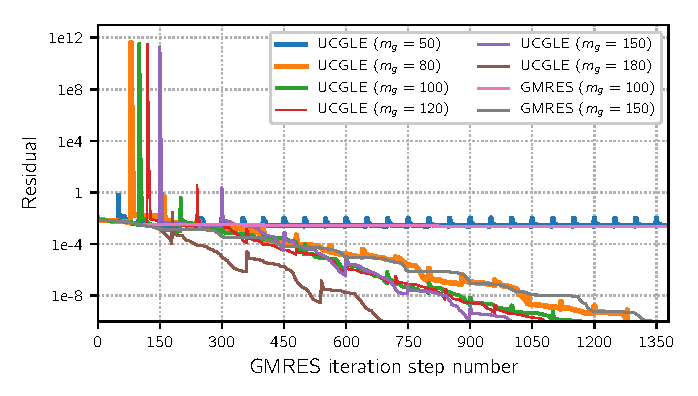
\includegraphics[width=6.2in]{fig/conv_ksp_gmres.eps}
	\caption{Evaluation of GMRES subspace size $m_g$ varying from $50$ to $180$. $l=10$, $lsa=10$, $freq=10$.}
	\label{fig:krylovsubspace}
\end{figure}

\begin{figure}[htbp]
	\centering
	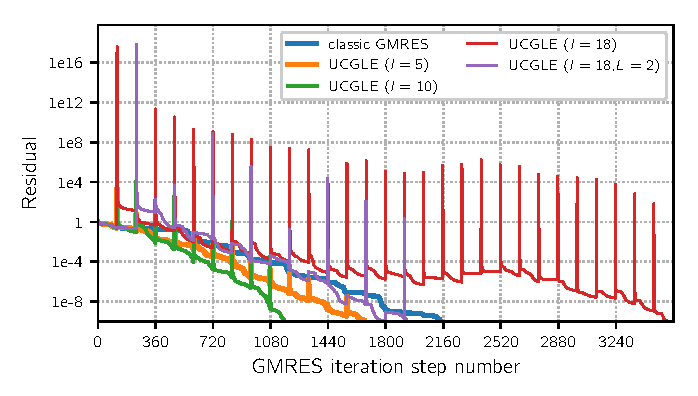
\includegraphics[width=6.2in]{fig/conv_power.eps}
	\caption{Convergence comparison of UCGLE method vs classic GMRES.}
	\label{fig:lsdegree}
\end{figure}

\begin{figure}[htbp]
	\centering
	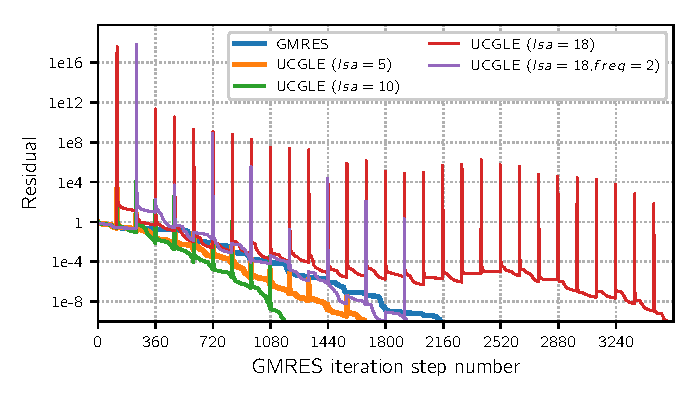
\includegraphics[width=6.2in]{fig/conv_lsappied.eps}
	\caption{Evaluation of LS applied times $lsa$ varying from $1$ to $25$, and $m_g=100$, $l=10$, $freq=1$. }
	\label{fig:Lsappliedtime}
\end{figure}

In conclusion, the Krylov subspace size of GMRES Component is a very important parameter of UCGLE. If this parameter is too small, it is difficult to get the convergence even with the LS polynomial preconditioning. It is not practical to use very large $m_g$ since the limitation of memory. Thus, it is essential to determine a good value of $m_g$ which is able to able to accelerate the convergence by LS polynomial. Moreover, UCGLE is able to converge with small Krylov subspace size that  classic GMRES cannot achieve the convergence with. The smaller Krylov subspace size is effective to reduce the number of global communications of SpMV inside Arnoldi reduction, and also the memory requirement.

\textbf{LS polynomial degree: }The parameter $l$  means the degree of  LS polynomial applied to the temporary residual of GMRES. If this polynomial is formulated by the polygon formatted by all the eigenvalues of operator $A$, the larger $l$ is, the better the approximation of solution will be, theoretically. In the experiments, $l$ are set respectively to be $5$, $10$, $15$, $20$ and $25$, and the parameters $m_g$, $lsa$, and $freq$ are respectively fixed as $100$, $10$ and $1$. Fig. \ref{fig:lsdegree} shows the convergence curves of all the tests. The influence of $l$ is clear, with the increase of $l$, the residual norm of the restart vector produced by LS polynomial will be enlarged, and GMRES Component will be accelerated. UCGLE with $l=25$ has more than 2$\times$ speedup than it with $l=5$.

In conclusion, $l$ is a very important parameter for the convergence of UCGLE. A good selection of this parameter should make a balance between the LS acceleration and the enlargement of the restarted residual norm. In practice, it is limited for choosing the degree of polynomial degree by the fact that the moment matrix $M_d$ becomes difficult to compute and to factor as the degree $l$ increases. A classical solution to this problem is to compound several times a small degree polynomial. This is done by performing the iteration from line \ref{lsastart} to \ref{lsaend} in Algorithm \ref{alg:gmres/ls-a} several times. We will evaluate this parameter $lsa$ in the next step.

\textbf{LS applied times: }The parameter LS applied times $lsa$ means the number of times the LS parameters will be applied to the temporary solution of GMRES Component before its restart after $m_g$ iterations.In the experiments, $lsa$ are set respectively to be $5$, $10$ and $18$, and the parameters $m_g$, $l$, and $freq$ are respectively fixed as $120$, $10$ and $1$.  An additional test is done with $l$ being $18$ and $freq$ being $2$.. Fig. \ref{fig:Lsappliedtime} shows the convergence curves of all the tests. Firstly, it is obvious that $lsa$ has an effect on the peaks for each time LS preconditioning. The greater it is, the bigger the peak will be. As talked in Section \ref{parameter analysis}, these peaks mean the Euclidean norm of restart vector produced by LS polynomial. By comparing the curves in Fig. \ref{fig:Lsappliedtime}, we can conclude that the augmentation of $lsa$ will accelerate the convergence of UCGLE. The influence of $lsa$ is clear, with the increase of $lsa$, the residual norm of the restart vector produced by LS polynomial will be enlarged. In the beginning, the test with $lsa=10$ performs better than $lsa=5$, since LS polynomial approximates better the dominant eigenvalues with a higher degree of the LS polynomial. However, if $lsa=18$, the residual norm is too large, the speedup of LS polynomial is covered, and the convergence might be slowed down.  For the larger $lsa$, we could select a larger $freq$, which might reduce the influence of too large residual norm caused by $lsa$. This means $lsa$ cannot be too large, otherwise it might lead to a too large norm of the residual of the restarted vector generated by LS polynomial preconditioning process and finally, damage the convergence. We will give an autotuning shceme for this parameter later in Chapter \ref{Parameters Autotuning}.

To conclude on the effect of this parameter, it is necessary to select the best value with considering the selection of the setting of LS polynomial power $l$. The two parameters seem particularly intricate together, and the choice of one will depend on the choice of the other. In the practical implementation, this parameter implies a series of SpMV and AXPY operations in parallel. The larger $l$ is, the more operations will be executed. Thus the more time will be occupied. The good selection of this parameter should make a balance between the reduction of iteration steps of GMRES components and additional time caused by these SpMV and AXPY operations.

\begin{figure}[htbp]
	\centering
	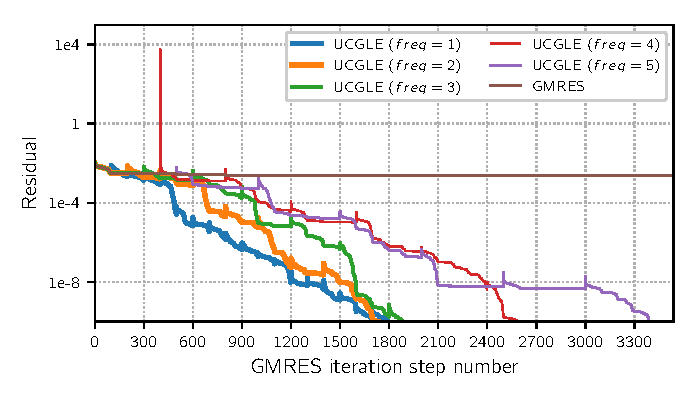
\includegraphics[width=6.2in]{fig/conv_lsfreq.eps}
	\caption{Evaluation of LS applied times $freq$.}
	\label{fig:Lsfreq}
\end{figure}

\begin{figure}[htbp]
	\centering
	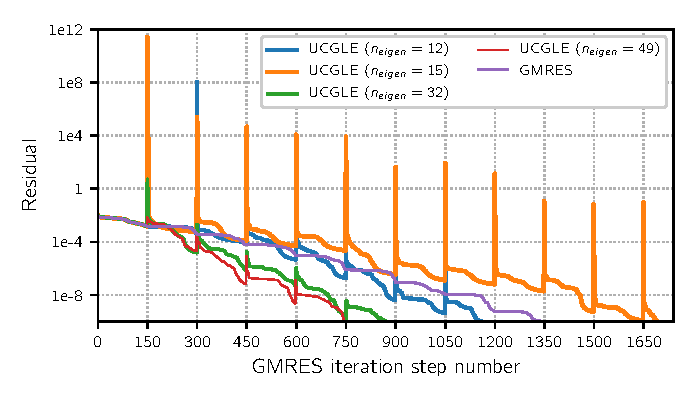
\includegraphics[width=6.2in]{fig/conv_eigenvalues.eps}
	\caption{Evaluation of eigenvalue number $n_{eigen}$.}
	\label{fig:vals}
\end{figure}

\textbf{LS frequency: }The preconditioning latency $freq$ represents the number of restarts between which a GMRES preconditioning will take place by the LS polynomial to the temporary solution. Also, we noticed in the previous experiments that after each preconditioning, a peak of the residual norm would be generated before the acceleration. This size of this peak depends on the influence of several parameters, and too large peak would damage the convergence.  In order to characterize the latency parameter, the Krylov subspace $m_g$, $lsa$and $l$ are respectively fixed as $100$, $10$, $10$, and $lsa$ ranges from $1$ to $5$. The results are shown in Fig. \ref{fig:Lsfreq}. For the cases with $freq$ being $1$, $2$ and $3$, their convergence performances are similar. If $freq$ is too large,  there are not enough LS preconditioning applied to UCGLE, and their convergence might be heavily slowed down. Ultimately, the latency parameter must be chosen to allow sufficient consideration of the preconditioning in the successive cycles at this stage while not being too important so that the convergence can continue to benefit from its effect at a satisfactory pace.

\textbf{Number of eigenvalues: } The parameter $n_{eigen}$ means the number of eigenvalues used to construct the polygon for the LS preconditioning. In the experiments, it is difficult to fix the number of approximated eigenvalues. Thus we select to change the Krylov subspace size of ERAM $m_g$ to control the number of eigenvalues applied to LS preconditioning. In the experiments,  the Krylov subspace $m_g$ is fixed as $150$. The parameters $lsa$, $l$, and $freq$ are respectively fixed as $10$, $10$ and $1$. The numbers of eigenvalues approximated by ERAM with different Krylov subspace sizes are respectively $12$, $15$, $32$ and $49$. The convergence comparison is given in Fig. \ref{fig:vals}. We can conclude that with the augmentation of the number of eigenvalues applied to the LS polynomial, the convergence of UCGLE can be accelerated, e.g., the test with $49$ eigenvalues has more than $2\times$ speedup comparing with the one with $12$ eigenvalues. Another phenomenon we can find is that the restart residual norm will be significantly decreased.  The reason is that with the much larger number of eigenvalues, the polygon constructed by them will be able to approximate the spectrum of operator matrix $A$ better. The solution of the min-max problem inside LS preconditioning is better, which results in the decrease of restart residual norm. The Krylov subspace size of ERAM cannot be as large as we want since it is necessary for the ERAM Component to approximate enough number of eigenvalues and send them to GMRES Component in time.

\subsection{Convergence Acceleration}

\begin{table}[htbp]
	\renewcommand{\arraystretch}{1.2}
	\caption{Test matrices information}
	\label{matget}
	\centering
	\begin{tabular}{x{4cm}|x{3cm}|x{3cm}|x{4cm}}
		\toprule
		\cellcolor{gray!50}Matrix Name& 	\cellcolor{gray!50}n & 	\cellcolor{gray!50}nnz & 	\cellcolor{gray!50}Matrix Type\\
		\midrule
		$matLine$  & \num[round-precision=2,round-mode=figures]{18000000} & \num[round-precision=2,round-mode=figures]{28823000} & non-Symmetric\\
		\hline
		$matBlock$  & \num[round-precision=2,round-mode=figures]{18000000} & \num[round-precision=2,round-mode=figures]{192160000} & non-Symmetric\\
		\hline
		$MEG1$ & \num[round-precision=4,round-mode=figures]{10240000} & \num[round-mode = places, scientific-notation = fixed, fixed-exponent = 9,round-precision = 2]{7270272000} & non-Hermitian\\
		\hline
		$MEG2$ & \num[round-precision=2,round-mode=figures]{5120000} & \num[round-mode = places, scientific-notation = fixed, fixed-exponent = 9,round-precision = 2]{3635136000} & non-Hermitian\\
		\bottomrule
	\end{tabular}
\end{table}

After the evaluation of different parameters on the convergence of UCGLE, in this section, we will compare the acceleration of UCGLE by LS polynomial with conventional preconditioned GMRES. We have selected four large-scale test matrices to evaluate the convergence speedup of UCGLE method. The test matrices $MEG1$ and $MEG2$ are built by performing several copies of the same small unsymmetrical matrix (utm300) onto the diagonal. For the generation of $MEG1$, several parallel lines with different values can be added to the off-diagonal. For $MEG2$, the first block column matrix as also filled by the small matrix utm300. The exact shapes of $MEG1$ and $MEG2$ are given in Fig. \ref{fig:matrixgenerator}. The test matrix $MEG3$ and the second matrix $MEG4$ are all generated by SMG2S with the prescribed eigenvalues distributed randomly inside an annulus with the different scales which is symmetric to the real axis in the complex plane. The information of the fours tests matrices is given in Table \ref{matget}. 

The convergence of UCGLE is compared with:

\begin{enumerate}[label=(\arabic*)]
	\item the restarted GMRES without preconditioning;
	\item restarted GMRES with Jacobi preconditioner;
	\item restarted GMRES with SOR preconditioner. 
\end{enumerate}

We select the Jacobi and SOR preconditioners for the experimentations because they are well implemented in parallel by PETSc. The GMRES restarted parameter for $MEG1$, $MEG2$, $MEG3$ and $MEG4$ are respectively 250, 280, 30 and 40.

\begin{table*}[htbp]
	\footnotesize
	\renewcommand{\arraystretch}{1.2}
	\caption{Summary of iteration number for convergence of $4$ test matrices using SOR, Jacobi, non preconditioned GMRES,UCGLE\_FT(G),UCGLE\_FT(G) and UCGLE: red $\times$ in the table presents this solving procedure cannot converge to accurate solution (here absolute residual tolerance \num[round-precision=2,round-mode=figures]{0.0000000001} for GMRES convergence test) in acceptable iteration number ($20000$ here).}
	\label{iterations}
	\centering
	\begin{tabular}{*{7}{c}}
		\toprule
		\cellcolor{gray!50}Matrix Name& 	\cellcolor{gray!50}SOR & 	\cellcolor{gray!50}Jacobi & 	\cellcolor{gray!50}No preconditioner & 	\cellcolor{gray!50}UCGLE\_FT(G) &	\cellcolor{gray!50}UCGLE\_FT(G) & 	\cellcolor{gray!50}UCGLE \\
		\midrule
		$MEG1$  & 1430 & \textcolor{red}{$\times$} & 1924 & 995 & 1073 & \cellcolor{yellow}900\\
		
		\cellcolor{gray!20}$MEG2$  & 	\cellcolor{gray!20}2481 & 	\cellcolor{gray!20}3579 & 	\cellcolor{gray!20}3027 & 	\cellcolor{gray!20}2048 & 	\cellcolor{gray!20}2005 & \cellcolor{yellow}1646\\
		
		$MEG3$ & 217 & 386 & 400 & 81 & 347 & \cellcolor{yellow}74\\
		
		\cellcolor{gray!20}	$MEG4$ & 	\cellcolor{gray!20}750 & 	\cellcolor{gray!20}\textcolor{red}{$\times$} & 	\cellcolor{gray!20}\textcolor{red}{$\times$} & 	\cellcolor{gray!20}82 & 	\cellcolor{gray!20}\textcolor{red}{$\times$} & \cellcolor{yellow}64\\
		\bottomrule
	\end{tabular}
\end{table*}

\begin{figure}[t]
	\centering
	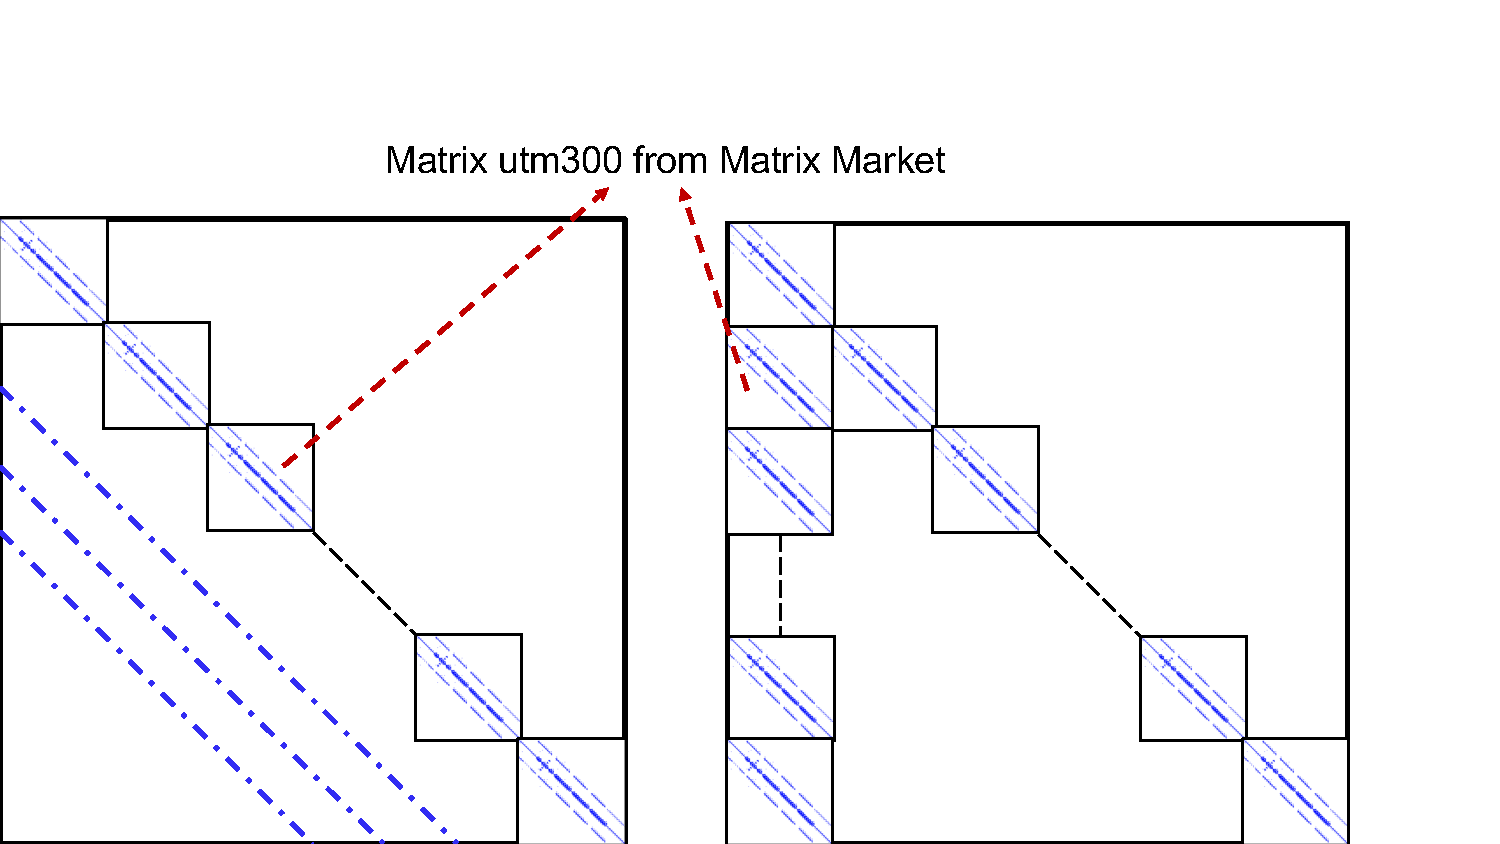
\includegraphics[width=0.8\linewidth]{fig/matrix_generator.pdf}
	\caption{Two strategies of large and sparse matrix generator by a original matrix utm300 of Matrix Market.}
	\label{fig:matrixgenerator}
\end{figure}

Fig \ref{fig:conv1}, Fig \ref{fig:conv2}, Fig \ref{fig:conv3} and Fig \ref{fig:conv4} present respectively the convergence experiments of $MEG1$, $MEG2$, $MEG3$ and $MEG4$. The numbers of iteration steps for convergence are given in Table \ref{iterations}. We find that UCGLE method has spectacular acceleration on the convergence rate comparing these conventional preconditioners. It has almost two times of acceleration for $MEG1$, $MEG2$ and $MEG3$, and more than 10 times of acceleration for $MEG4$ than the conventional preconditioner SOR. The SOR preconditioner is already much better than the Jacobi preconditioner for the test matrices.

\begin{figure}[htbp]
	\centering
	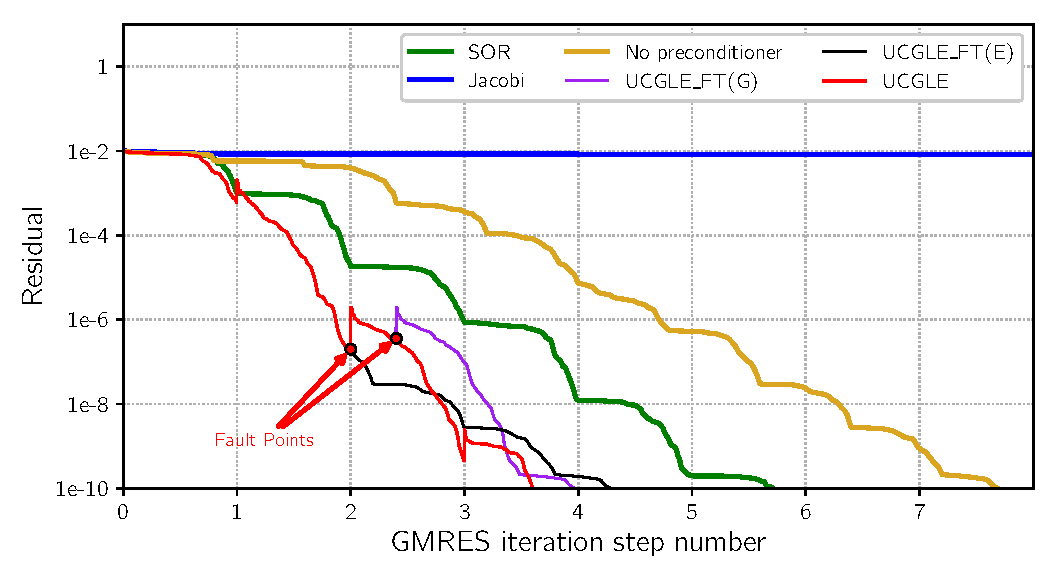
\includegraphics[width=0.99\linewidth]{fig/convergence1.eps}
	\caption{$MEG1$: convergence comparison of UCGLE method vs conventional GMRES}
	\label{fig:conv1}
\end{figure}

\begin{figure}[htbp]
	\centering
	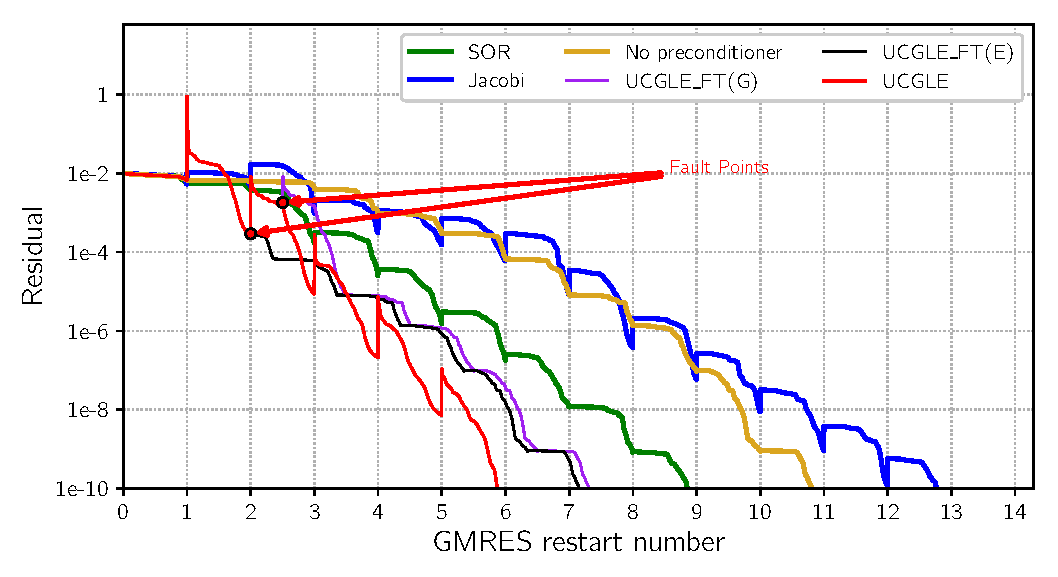
\includegraphics[width=0.99\linewidth]{fig/convergence2.eps}
	\caption{$MEG2$: convergence comparison of UCGLE method vs conventional GMRES}
	\label{fig:conv2}
\end{figure}

\begin{figure}[htbp]
	\centering
	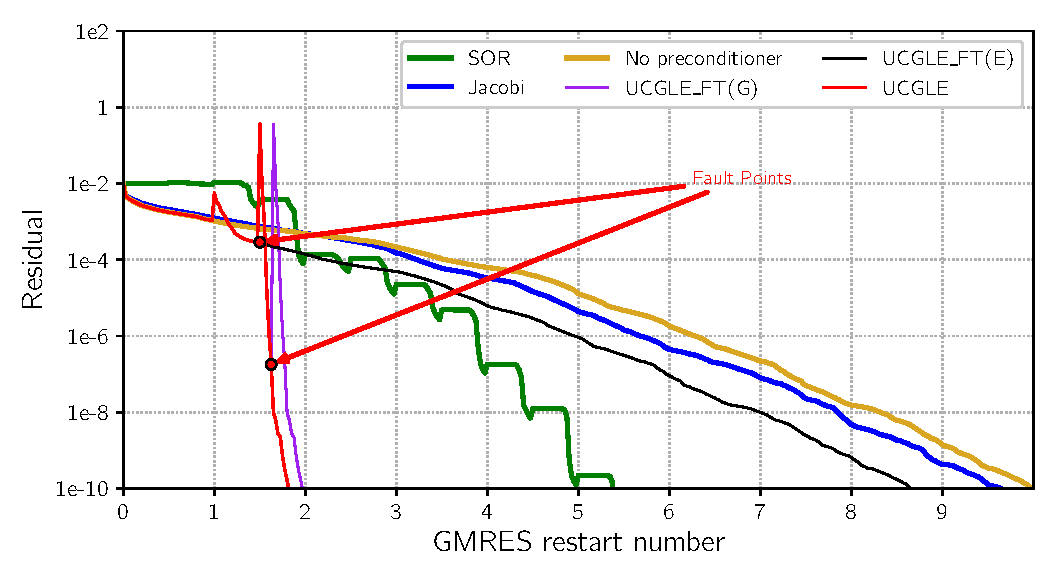
\includegraphics[width=0.99\linewidth]{fig/convergence3.eps}
	\caption{$MEG3$: convergence comparison of UCGLE method vs conventional GMRES}
	\label{fig:conv3}
\end{figure}

\begin{figure}[htbp]
	\centering
	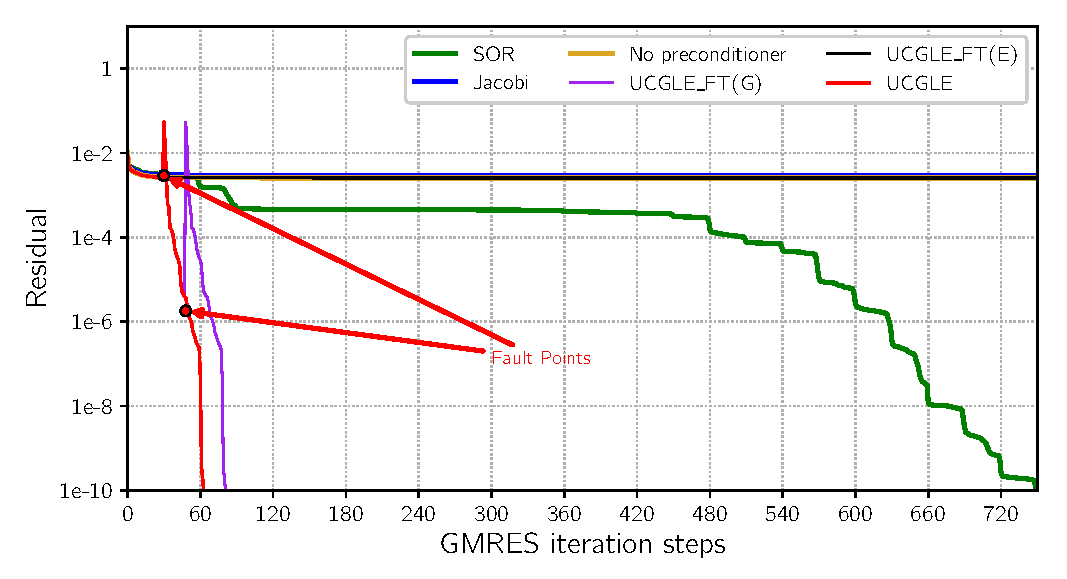
\includegraphics[width=0.99\linewidth]{fig/convergence4.eps}
	\caption{$MEG4$: convergence comparison of UCGLE method vs conventional GMRES}
	\label{fig:conv4}
\end{figure}

\subsection{Fault Tolerance Evaluation}

The fault tolerance of UCGLE is studied by the simulation of the loss of either GMRES or ERAM Components. UCGLE\_FT(G) in Fig. \ref{fig:conv1}, Fig. \ref{fig:conv2}, Fig. \ref{fig:conv3} and Fig. \ref{fig:conv4} represents the fault tolerance simulation of GMRES, and UCGLE\_FT(E) implies the fault tolerance simulation of ERAM. 

The failure of ERAM Component is simulated by fixing the execution loop number of ERAM algorithm, in this case, ERAM exits after a fixed number of solving procedures. We mark the ERAM fault points of the two test matrices in Fig. \ref{fig:conv1}, Fig. \ref{fig:conv2},  Fig. \ref{fig:conv3} and Fig. \ref{fig:conv4} : respectively $500$, $560$, $60$ and $30$ iteration step for each case. The UCGLE\_FT(E) curves of the experimentations show that GMRES Component will continue to resolve the systems without LS acceleration. Table \ref{iterations} shows that the iteration number for convergence of UCGLE\_FT(E) is greater than the normal UCGLE method but less than the GMRES method without preconditioning.

The failure of GMRES Component is simulated by setting the allowed iteration number of GMRES algorithm to be much smaller than the needed iteration number for convergence. The values of these cases are respectively $600$, $700$, $70$ and $48$. They are also marked in Fig. \ref{fig:conv1}, Fig. \ref{fig:conv2}, Fig. \ref{fig:conv3} and Fig. \ref{fig:conv4}. We can find that after the quitting of GMRES Component without the finish of its task, ERAM computing units will automatically take over the jobs of GMRES component. The new GMRES resolving procedure will use the temporary solution $x_m$ as a new restarted initial vector received asynchronously from the previous restart procedure of GMRES Component before its failure. In this case, ERAM Component no longer exists. Thus the resolving task can be continued as the classic GMRES without LS preconditioning. In  Fig. \ref{fig:conv1}, Fig. \ref{fig:conv2}, Fig. \ref{fig:conv3} and Fig. \ref{fig:conv4}, we can find the difference between UCGLE\_FT(E) and UCGLE\_FT(G). In UCGLE\_FT(G), the new GMRES Component takes $x_m$ of previous restart procedure. Thus it will repeat the iteration steps of previous restart iterations until the failure of GMRES. Another fact of UCGLE\_FT(G) which cannot be concluded, but can be easily obtained, is that the resolving time will be different if the computing unit numbers of previous GMRES and ERAM Components are different.

\subsection{Impacts of Spectrum on Convergence}

The Least Squares Polynomial uses the dominant eigenvalues to accelerate the convergence of iterative methods. With the help of SMG2S, we could study the impacts of spectral distribution on the convergence of UCGLE. In this section, we evaluate the acceleration of UCGLE with eight types of spectrum, they are generated by the functions listed in Table \ref{specgetfunc}. The dimension for all eight test matrices is fixed as 2000. The experimental results are given in Fig. \ref{fig:spec} and Fig. \ref{fig:specspec}. For all the tests, the Krylov subspace size $m_a$ for ERAM Component is limited. Thus the accuracy of approximated eigenvalues is also low. However, the speedup of LS polynomial preconditioning is still splendid. The purpose to limit $m_a$ is to make sure generate enough eigenvalues for the first time restart of GMRES Component inside UCGLE. If this subspace size is too large, or the conditions for the eigenvalues to be accepted are too strict, there will be no acceleration by LS polynomial preconditioning.

\begin{table}[htbp]
	\scriptsize
	\renewcommand{\arraystretch}{2.0}
	\caption{Spectrum Generation Functions: the size of all spectra is fixed as $N=2000$, $i \in 0, 1,\cdots, N-1$ is the indices for the eigenvalues.}
	\label{specgetfunc}
	\centering
	\begin{tabular}{x{0.6cm}|x{7.6cm}|x{6.4cm}}
		\toprule
		\cellcolor{gray!50}$N^o$& 	\cellcolor{gray!50}real part & 	\cellcolor{gray!50}imaginary part \\
		\midrule
		I  &$0.6 + (rand (0,0.01)+0.55)\cos(2\pi i/N-\pi)$&  $(rand (0,0.01)+0.1)\sin(2\pi i/N-\pi)$\\
		\hline
		\cellcolor{gray!20}II  & \cellcolor{gray!20}$0.3 + (rand (0,0.01)+0.55)\cos(2\pi i/N-\pi)$&  \cellcolor{gray!20}$(rand (0,0.01)+0.1)\sin(2\pi i/N-\pi)$\\
		\hline
		III &$-0.6 + (rand (0,0.01)+0.55)\cos(2\pi i/N-\pi)$&  $(rand (0,0.01)+0.1)\sin(2\pi i/N-\pi)$ \\
		\hline
		\cellcolor{gray!20}IV &\cellcolor{gray!20}$0.6 + (rand (0,0.01)+0.55)\cos(4\pi i/N-\pi)$&\cellcolor{gray!20}$\pm0.2\pm(rand (0,0.01)+0.1)\sin(4\pi i/N-\pi)$\\
		\hline
		V  &$0.006 + rand (0,0.5)$ & $0.0$\\
		\hline
		\cellcolor{gray!20}VI  & \cellcolor{gray!20}$-0.006 + rand (0,0.5)$ & \cellcolor{gray!20}$0.0$\\
		\hline
		\multirow{2}{*}{VII}&$60.0 + (rand (0,0.0001)+0.00012)\cos(2\pi i/N-\pi) \ \forall i < 50$&$(rand (0,0.0001)+0.00012)\sin(2\pi i/N-\pi) \ \forall i < 50$ \\
		&$0.6 + (rand (0,0.01)+0.55)\cos(2\pi i/N-\pi) \ \forall i \geq 50$&$(rand (0,0.01)+0.1)\sin(2\pi i/N-\pi)\ \forall i \geq 50$ \\
		\hline
		\cellcolor{gray!20}&\cellcolor{gray!20}$-60.0 - (rand (0,0.0001)+0.00012)\cos(2\pi i/N-\pi) \ \forall i < 50$&\cellcolor{gray!20}$(rand (0,0.0001)+0.00012)\sin(2\pi i/N-\pi) \ \forall i < 50$ \\
		\multirow{-2}{*}{\cellcolor{gray!20}VIII}&\cellcolor{gray!20}$-0.6 - (rand (0,0.01)+0.55)\cos(2\pi i/N-\pi) \ \forall i \geq 50$&\cellcolor{gray!20}$(rand (0,0.01)+0.1)\sin(2\pi i/N-\pi)\ \forall i \geq 50$ \\
		\bottomrule
	\end{tabular}
\end{table}

The generated spectrum I is quasi-symmetric to the real axis, and all the real parts of these eigenvalues are positive, shown as Fig. \ref{spec1}. The Ritz values approximated by ERAM are marked as the red cross in the figure. The parameters $l$ and $lsa$ for the LS polynomial preconditioning are all set to be $10$. In the experiments, for UCGLE with Krylov subspace size of GMRES Component $m_g=20$, it has more than $3\times$ speedup over the conventional GMRES for the convergence. But for the case UCGLE with much Krylov subspace size $m_g=80$ in GMRES Component, it only has about $1.4\times$ over the conventional GMRES. In fact, for all the matrices with a spectral distribution similar to spectrum I, the LS polynomial preconditioning is always very effective, and it is better to benefit from this preconditioning as soon as possible. Hence, GMRES Component with smaller $m_g$ might converge much more rapidly than the case with larger $m_g$, since it can profit the LS polynomial preconditioning in time.

The spectrum II is also quasi-symmetric to the real axis, its shape is near an ellipse. The real part of some eigenvalues in the spectrum is positive, and for the others, the real part is negative, shown as Fig. \ref{spec2}. In this case, UCGLE cannot achieve the convergence even with much larger Krylov subspace size $m_g=200$. When the original point is inside the spectrum of the operator matrix. As we presented in Chapter \ref{Krylov Subspace Methods}, the maximum-minimum problem of LS polynomial method cannot be solved. In the current implementation of LS polynomial preconditioning, for most cases with the origin point inside spectrum, UCGLE with LS polynomial preconditioning is not applicable.

The spectrum III in Fig. \ref{spec3} is also quasi-ymmetric to the real axis, and the real part of all the eigenvalues are negative. The Ritz values approximated by ERAM Component are also marked as the red cross in the figure. This case is similar to the one in Fig. \ref{spec1}. The acceleration of LS polynomial preconditioning inside UCGLE is obvious, and this kind of spectral distribution is suitable for the polynomial preconditioning.

\begin{figure*}[htbp]
	\centering
	\subfloat[Spectral Distribution I: matrix size $= 2000$, $l=10$, $lsa=10$, $freq=1$.]{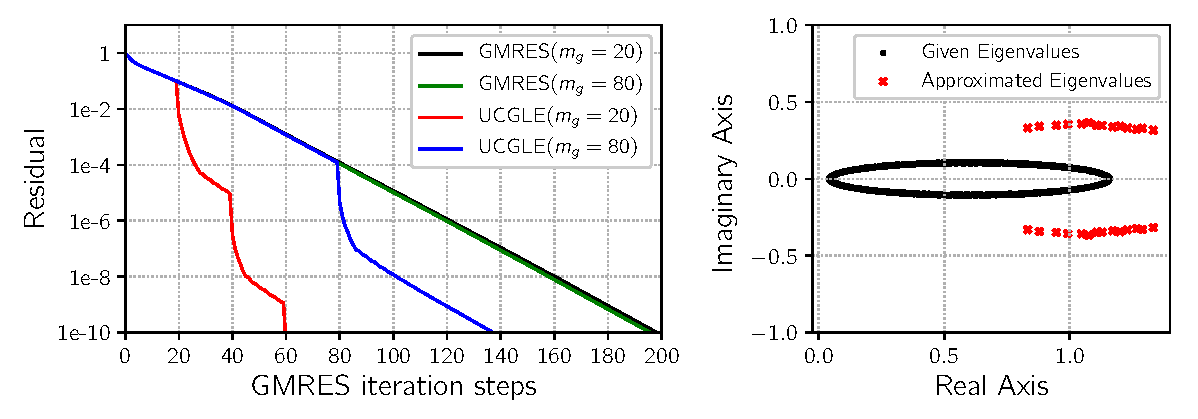
\includegraphics[width=.96\linewidth]{fig/spec3.eps}%
		\label{spec1}}
	\vspace{-0.06in}
	\subfloat[Spectral Distribution II: matrix size $= 2000$, $m_g=200$, $l=10$, $lsa=10$, $freq=1$.]{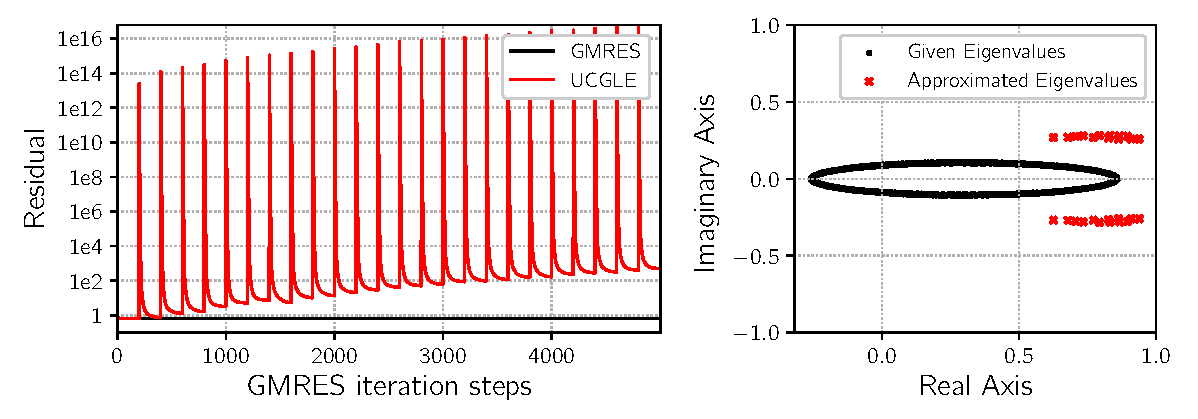
\includegraphics[width=.96\linewidth]{fig/spec4.eps}%
		\label{spec2}}
	\vspace{-0.06in}
	\subfloat[Spectral Distribution III: matrix size $= 2000$, $l=10$, $lsa=10$, $freq=1$.]{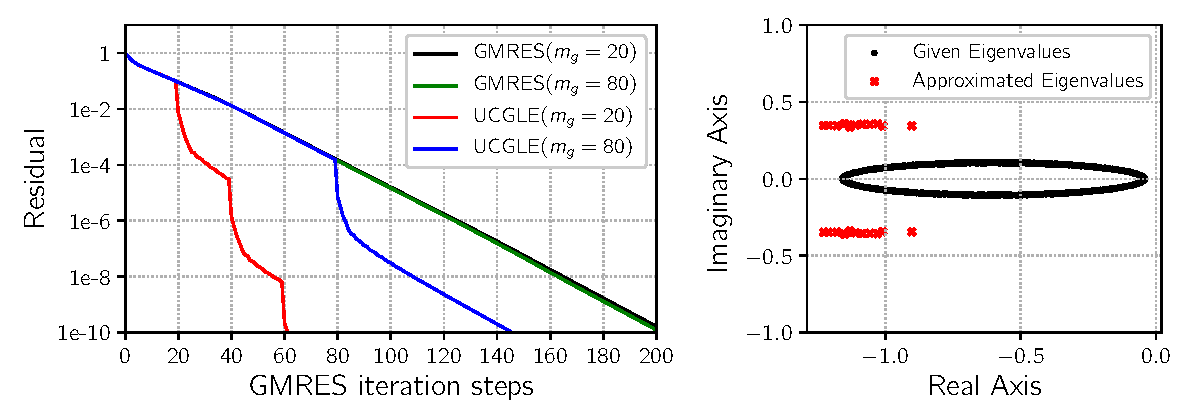
\includegraphics[width=.96\linewidth]{fig/spec5.eps}%
		\label{spec3}}
	\vspace{-0.06in}
	\subfloat[Spectral Distribution IV: matrix size $= 2000$, $m_g=20$, $l=10$, $lsa=10$, $freq=1$.]{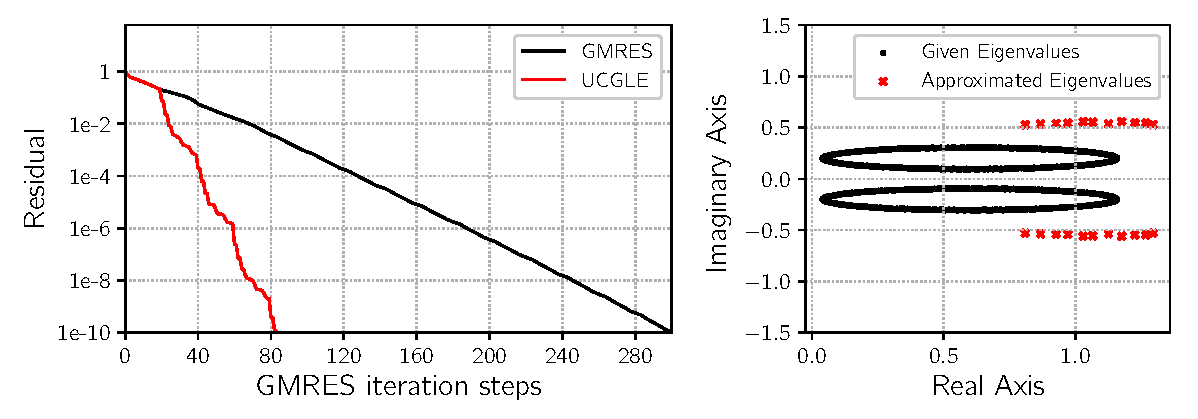
\includegraphics[width=.96\linewidth]{fig/spec8.eps}%
		\label{spec4}}
	\caption{Impacts of Spectrum on Convergence.}
	\label{fig:spec}
\end{figure*}

\begin{figure*}[htbp]
	\centering
	\subfloat[Spectral Distribution V: matrix size $= 2000$, $m_g=10$, $l=10$, $lsa=10$, $freq=1$.]{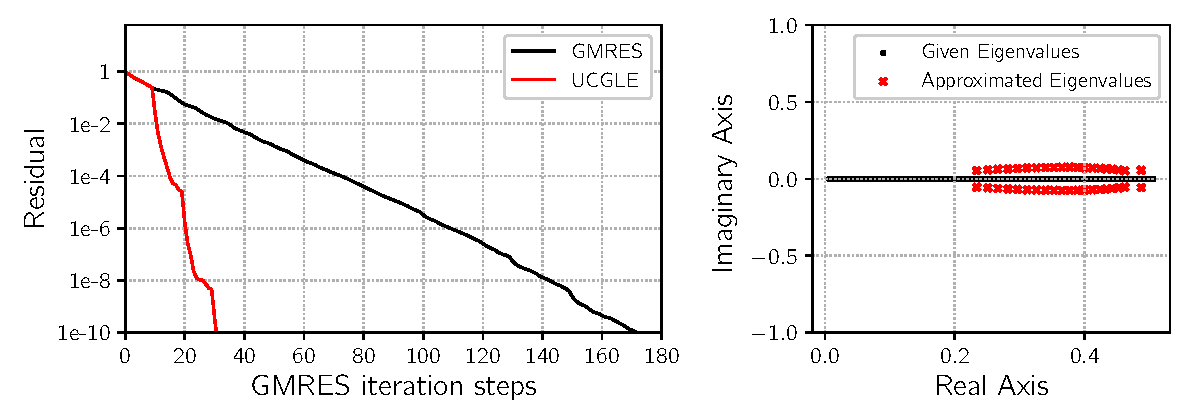
\includegraphics[width=.96\linewidth]{fig/spec1.eps}%
		\label{spec5}}
	\vspace{-0.06in}
	\subfloat[Spectral Distribution VI: matrix size $= 2000$, $m_g=50$, $lsa=10$, $freq=1$.]{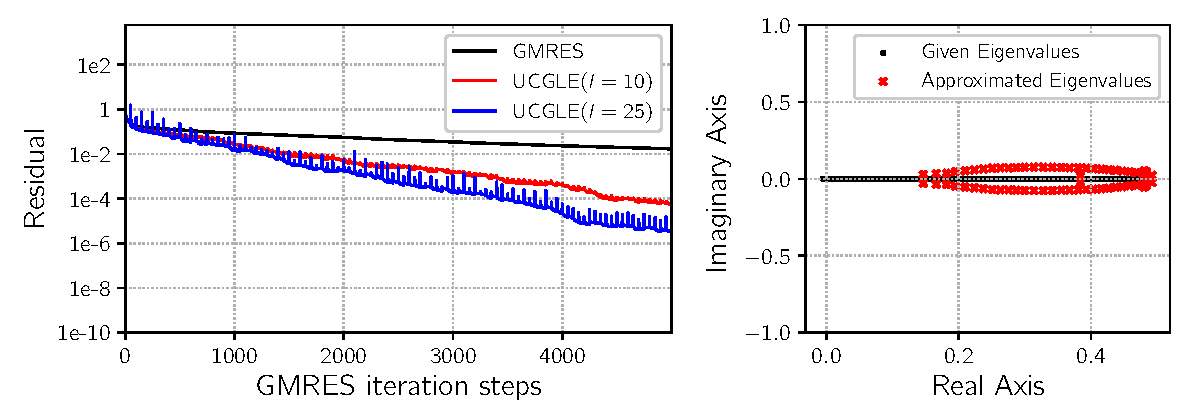
\includegraphics[width=.96\linewidth]{fig/spec2.eps}%
		\label{spec6}}
	\vspace{-0.06in}
	\subfloat[Spectral Distribution VII: matrix size $= 2000$, $m_g=20$, $l=10$, $lsa=10$, $freq=1$.]{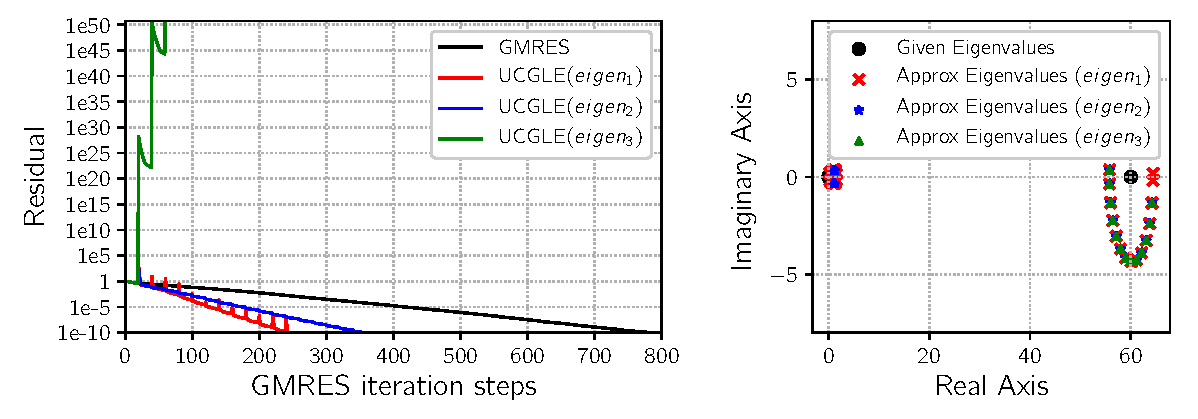
\includegraphics[width=.96\linewidth]{fig/spec6.eps}%
		\label{spec7}}
	\vspace{-0.06in}
	\subfloat[Spectral Distribution VIII: matrix size $= 2000$, $m_g=20$, $l=10$, $lsa=10$, $freq=1$.]{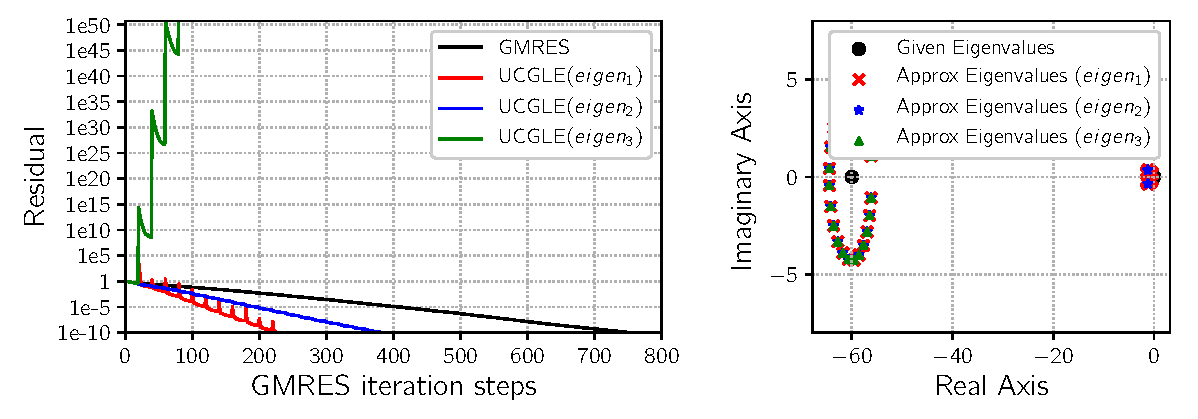
\includegraphics[width=.96\linewidth]{fig/spec7.eps}%
		\label{spec8}}
	\caption{Impacts of Spectrum on Convergence.}
	\label{fig:specspec}
\end{figure*}


The spectrum IV in Fig. \ref{spec4} consists of two ellipses which are symmetric to the real axis, and the real part of all eigenvalues are positive. The Ritz values approximated by ERAM are marked as the red cross in the figure. We could conclude that UCGLE is suitable for this case with almost $4\times$ speedup comparing the conventional GMRES. 

The spectrum V in Fig. \ref{spec5} is generated in random with all the eigenvalues located on the real axis, the imaginary part of all eigenvalues is zero, and the real part is positive. The Ritz values approximated by ERAM are complex, which are also marked by the red cross in this figure. UCGLE has more than $6\times$ speedup for this spectrum, comparing with the conventional GMRES.

The spectrum VI in Fig. \ref{spec6} is also generated in random on the real axis using a different shift value with the one in  Fig. \ref{spec5}. The imaginary part of all the eigenvalues is also zero. However, the real part of a small number of eigenvalues are negative, and the real part of the others are positive. Since the origin point is inferior to the spectrum, the convergence both for GMRES and UCGLE is hard to be obtained. However, UCGLE has still a little speedup over the conventional GMRES. If we enlarge the degree of LS preconditioning polynomial from $10$ to $25$, we can continue to have some acceleration.

The spectrum VII and VIII  in Fig. \ref{spec7} and Fig. \ref{spec8} are also quasi-symmetric to the real axis, and the real parts of the eigenvalues for the two spectra are respectively all positive and negative. The two spectra are generated with a special manner which makes the eigenvalues be grouped into two seprate clustered set with a relative long distance in the real-imaginary plane. With the change of Krylov subspace $m_a$ of ERAM, different numbers of eigenvalues can be approximated. Three cases in the experiments are denoted as $eigen_1$, $eigen_2$ and $eigen_3$, which are marked with different colors in Fig. \ref{spec7} and Fig. \ref{spec8}. In the experiments, $eigen_1$ and $eigen_2$ are the Ritz values which approximate a few eigenvalues in both two clustered group. However, $eigen_3$ are only the Ritz values which approximate the eigenvalues in only one clustered group (the right clustered group in Fig. \ref{spec7}, and the left clustered group in Fig. \ref{spec8}). $eigen_1$ approximates more eigenvalues in the both two clustered group than $eigen_2$.  We could conclude from  Fig. \ref{spec7} and Fig. \ref{spec8} that UCGLE with $eigen_1$ converge the most rapid, with about $3\times$ speedup than the conventional GMRES, $eigen_2$ has almost $2\times$ speedup, and $eigen_3$ diverge quickly in a few iteration steps. The reason is that $eigen_3$ approximates only one clustered group, and the polygon constructed by $eigen_3$ cannot represent the real spectral distribution, which makes the norm of residual vector generated by LS poynomial explode in short time, and it is impossible to achieve the convergence.

We can conclude that:

\begin{enumerate}[label=(\arabic*)]
	\item If the real part of the eigenvalues of the operator matrix is all positive or negative, and the spectrum is (quasi-)symmetric to the real axis, UCGLE can always accelerate the convergence.
	
	\item If the real part for some eigenvalues of the operator matrix is positive and for some is negative, the divergence of UCGLE can be easily achieved, UCGLE is not suitable for this case; however, it might exist some particular matrices which can obtain the speedup of UCGLE.
	
	\item For the matrices with a good spectral distribution as we talked in (1), the approximated eigenvalues need not to be too accurate to allow the speedup by UCGLE.
	
	\item The more eigenvalues approximated to construct the LS polynomial, the more acceleration UCGLE will achieve.
	
    \item For the eigenvalues distributed into the different clustered groups with their real part to be all positive or all negative, much more Ritz values are required for constructing the LS polynomial preconditioning. At least, the Ritz values should be able to represent the different clustered groups of eigenvalues. If the different groups of clustered eigenvalues are very discrete, it is difficult for ERAM to approximate all of them with small Krylov subspace size. Thus the implementation of UCGLE with multiple ERAM Components is required. Each ERAM is executed with different shift value to approximate the different parts of eigenvalues with thick restarting. The difficulties are: 1) the implementation of current manager engine does not allow adding more computational components since it is implemented by statically dividing MPI\_COMM\_World into four communicators; 2)  for the matrices of real applications, we cannot know the clustering situations of their spectra. Thus the selection of shift value for different ERAM Components seems somehow blind. It is necessary to have the mechanism which can predict the distribution of clustered groups of eigenvalues with a relatively long distance.
	
    \item New model should be proposed for the eigenvalues with both positive and negative real parts. One possible solution is to implement two separate LSP components to construct two LS polynomials by the Ritz values with the positive and negative real part and exclude the origin point. Denote the two constructed residual polynomial to be $R_{d}$ and $R'_{d'}$. $R_{d}$ is constructed with $m$ dominant eigenvalues with positive real parts, and $R'_{d'}$ is constructed with $m'$ eigenvalues with largest magnitude and negative real part. The restarted residual vector generated by two LS polynomials should be
	
	\[
	r = \sum_{i=1}^{m}\rho_i R_d(\lambda_i)u_i + \sum_{i=m+1}^{n}\rho_i R_d(\lambda_i)u_i+\sum_{j=1}^{m'}\rho_j R'_{d'}(\lambda_j)u_j + \sum_{j=m'+1}^{n}\rho_j R'_{d'}(\lambda_j)u_j.
	\]
	
\end{enumerate}

\begin{figure}[htbp]
	\centering
	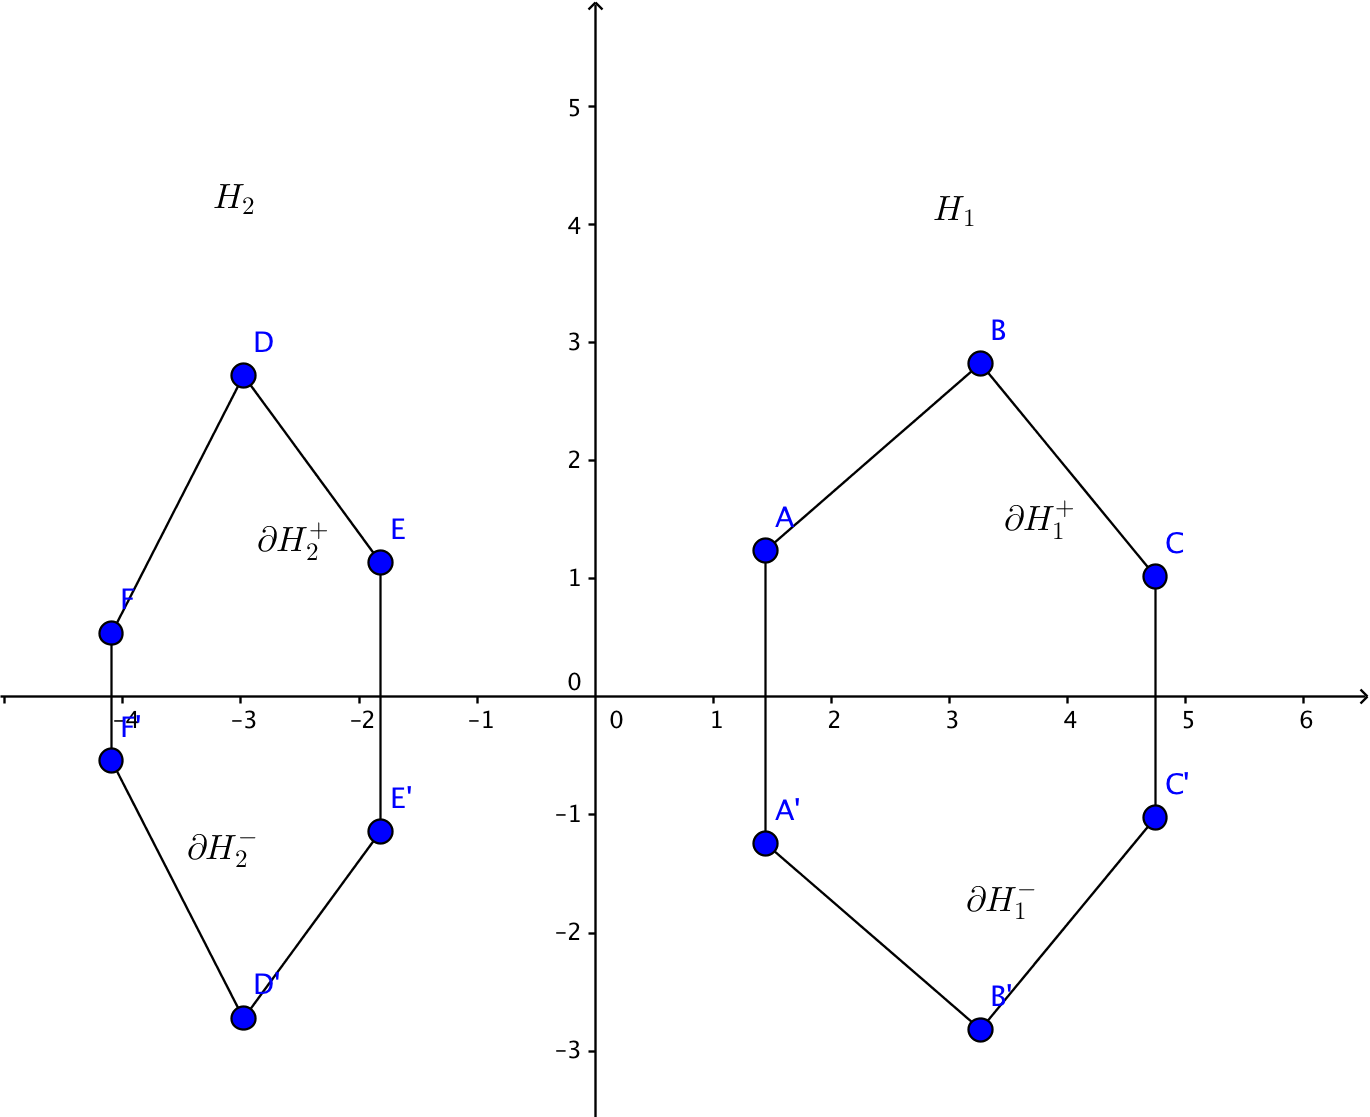
\includegraphics[width=0.8\linewidth]{fig/real-imaginary.png}
	\caption{Polygone region $H$ with real part of eigenvalues positive and negative.}
	\label{fig:imag-complex}
\end{figure}

\subsection{Scalability Evaluation}

When solving large-scale linear systems on the modern supercomputing platforms, the main concern of the conventional preconditioned Krylov methods is the cost of global communications and synchronization overheads. We select the test matrix $MEG1$ for the scalability evaluation. The average time cost per iteration of these methods is computed by a fixed number of iterations. Time per iteration is suitable for demonstrating scaling behavior. The scaling performance of UCGLE is evaluated both on Tianhe-2 and ROMEO.

\begin{figure*}[htbp]
	\centering
	\subfloat[]{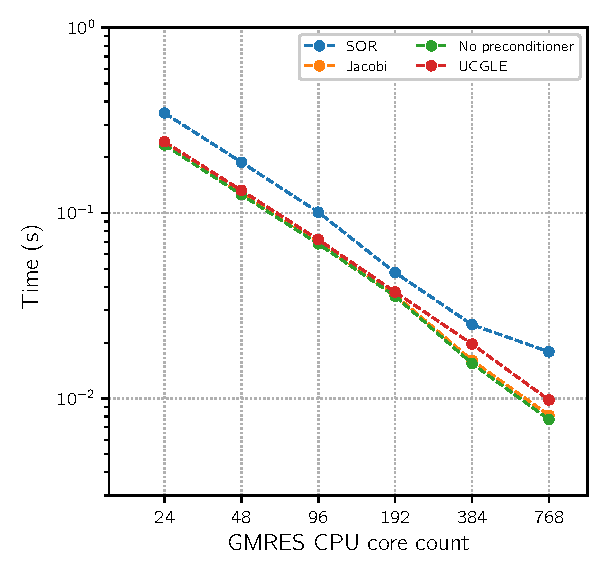
\includegraphics[width=.499\linewidth]{fig/scalable_th.eps}%
		\label{fig_th1_case}}
	\subfloat[]{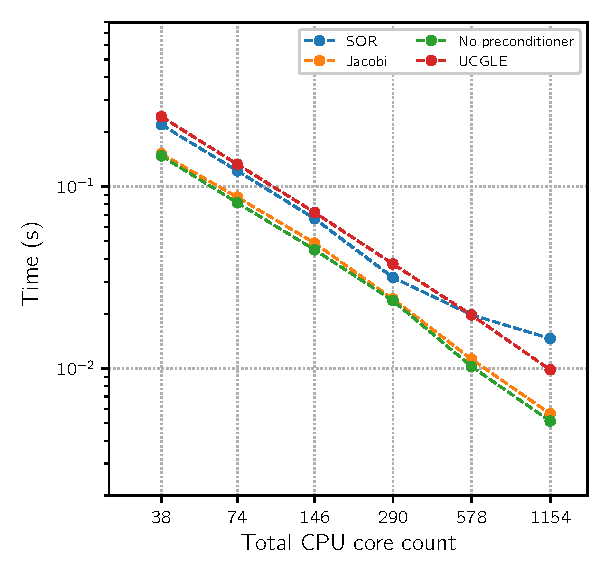
\includegraphics[width=.499\linewidth]{fig/scalable_complet.eps}%
		\label{fig_th2_case}}
	~\\
	\subfloat[]{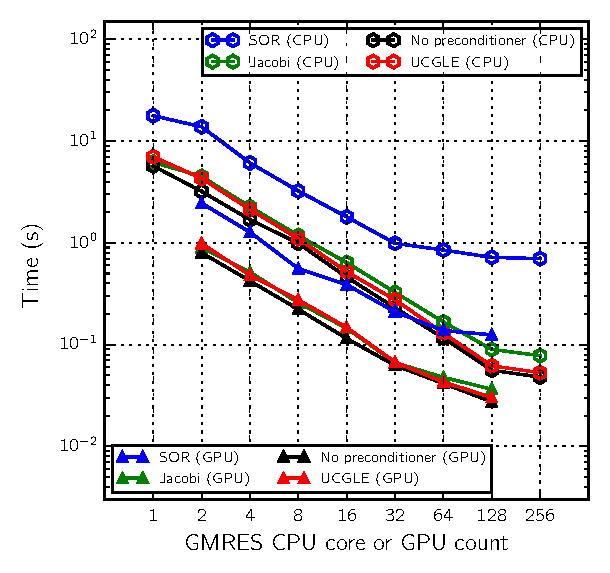
\includegraphics[width=.499\linewidth]{fig/scalable_romeo.eps}%
		\label{fig_romeo1_case}}
	\subfloat[]{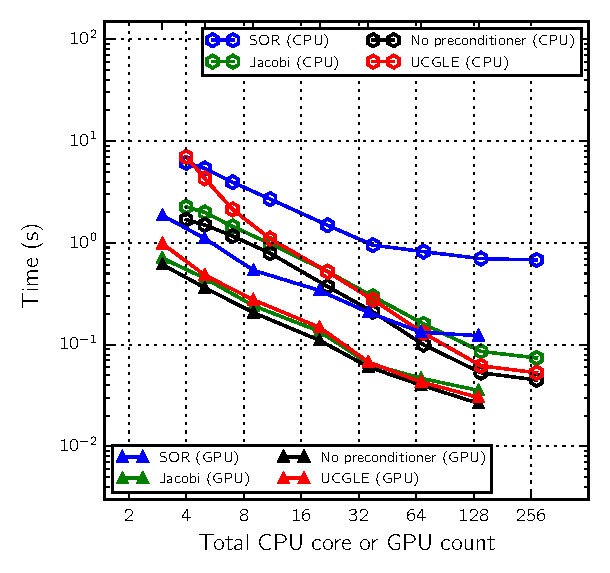
\includegraphics[width=.499\linewidth]{fig/scalable_complet_romeo.eps}%
		\label{fig_romeo2_case}}
	\caption{Scalability per iteration comparison of UCGLE with GMRES with or without preconditioners on Tianhe-2 and ROMEO. A base 10 logarithmic scale is used for Y-axis of (a); a base 2 logarithmic scale is used for Y-axis of (b).}
	\label{fig:myfig}
\end{figure*}

For the evaluation of UCGLE on ROMEO with CPUs, the core number of GMRES Component is set respectively to be 1, 2, 4, 8, 16, 32, 64, 128, 256, and both the core number of LS Component and Manager Component is 1. ERAM Component should ensure to supply the approximated eigenvalues in time for each time restart of GMRES Component. Thus the core number is respectively 1, 1, 1, 1, 4, 4, 4, 10, 16, referring to different GMRES Component core number. For the evaluation with multi-GPU on ROMEO, both LS Component and Manager Component allocate only one core on CPU. The GPU number of GMRES Component is set respectively to be 2, 4, 8, 16, 32, 64, 128, with the GPU number of ERAM Component respectively 1, 1, 1, 4, 4, 4, 8. The computing resource number of classic and preconditioned GMRES always keeps the same with the core number of GMRES Component in UCGLE method. Thus it ranges from 1 to 256 for CPU performance evaluation, and from 2 to 128 for GPU performance evaluation.

For the evaluation of UCGLE on Tianhe-2 with CPUs, the core number of GMRES Component is set respectively to be 24, 48, 96, 192, 384, 768, and both the core number of LS Component and Manager Component is 1. Thus we select the core number is respectively 16, 32, 64, 128, 256, 512 referring to different GMRES Component core number. The GMRES core number of conventional GMRES is equal to the one of GMRES Component in UCGLE.

In Fig. \ref{fig_th1_case} and Fig. \ref{fig_romeo1_case}, we can find that these methods have good scalability with the augmentation of computing units except the SOR preconditioned GMRES. The classic GMRES has the smallest time cost per iteration. The Jacobi preconditioner is the simplest preconditioning form for GMRES, and its time cost per iteration is similar to the classic GMRES. The GMRES with SOR preconditioner has the largest time cost per iteration since SOR preconditioned GMRES has the additional matrix-vector and matrix-matrix multiplication operations in each step of the iteration. These operations have global communication and synchronization points. The communication overhead makes the SOR preconditioned GMRES more easily lose its good scalability with the augmentation of computing unit number. There is not much difference between the time cost per iteration of classic GMRES and UCGLE with the help of the asynchronous communication implementation of UCGLE method. Since the resolving part and preconditioning part of UCGLE work independently, its global communication and synchronize points is similar to the classic GMRES without preconditioning. That is the benefits UCGLE's asynchronous communication. 

Since UCGLE requires additional computing units for the manager engine, LS Component and especially ERAM Component, it is necessary to compare UCGLE with other methods when the total computing resource number of UCGLE and other methods keeps the same computing resource number of UCGLE and other methods the same. Thus we have tested the classic and conventional preconditioned GMRES on ROMEO with the CPU core number fixed respectively as 4, 5, 7, 11, 22, 38, 70, 140, 274 and the GPU number fixed respectively as 3, 5, 9, 20, 36, 68, 136, referring to the previous scaling performance evaluation of UCGLE. In the evaluation on the GPU cluster, the two CPUs for LS Component and Manager Component have been ignored because they have a minor influence. For the evaluation on Tianhe-2, the computing unit number is fixed as 38, 74, 146, 290, 578, 1154. The performance comparison on Tianhe-2 and ROMEO are respectively given as Fig. \ref{fig_th2_case} and Fig. \ref{fig_romeo2_case} . We can find that if the computing resource number is small, the time per iteration of classic and conventional preconditioned GMRES is much better than UCGLE since the latter allocates extra computing resources for other components. With the augmentation of computing resources, the scalability of the SOR preconditioned GMRES trends to be bad, and the average time cost per iteration of UCGLE method tends to be better than the SOR preconditioned GMRES with good scalability. Although the scalability of classic and Jacobi is good, and their time per iteration is smaller than UCGLE, but since UCGLE can accelerate the convergence of solving linear systems, thus better performance can be expected. For test matrix $MEG1$ on ROMEO, UCGLE method has similar speedup on the solving time per iteration comparing with the classic GMRES when the computing resource number is larger than 22 for CPUs and larger than 5 for GPUs, but it can decrease significantly more than 5× iteration step number for the convergence, thus about 5× acceleration for the time of the whole resolution. In the end, the better performance of UCGLE method comparing with other methods can be concluded.

\section{Conclusion}

In this chapter, we have presented a distributed and parallel method UCGLE for solving large-scale non-Hermitian linear systems. This method has been implemented with asynchronous communication among different computation components. In the experimentation, we observed that UCGLE method has following features: 1) it has significant acceleration for the convergence than the conventional preconditioners as SOR and Jacobi; 2) the spectrum of different linear systems has influence on its improvement of convergence rate; 3) it has better scalability for the very large-scale linear systems; 4) it is able to speed up using GPUs; 5) it has the fault tolerance mechanism facing the failure of different computation components. We conclude that UCGLE method is a good candidate for emerging large-scale computational systems because of its asynchronous communication scheme, its multi-level parallelism, its reusability and fault tolerance, and its potential load balancing. The coarse grain parallelism among different computation components and the medium/fine grain parallelism inside each component can be flexibly mapped to large-scale distributed hierarchical platforms.

\clearemptydoublepage